\documentclass[11pt]{My_preprint}
%DIF LATEXDIFF DIFFERENCE FILE
%DIF DEL ../The_hybride_model_old.tex   Wed Sep 11 13:51:16 2024
%DIF ADD ../The_hybride_model_new.tex   Thu Sep 12 16:22:28 2024


\title{Averaged equations for disperse two-phase flow with interfacial transport}

\author[1,2]{Nicolas Fintzi}
\author[1]{Jean-Lou Pierson}
\affil[1]{IFP Energies Nouvelles, Rond-point de l'echangeur de Solaize, 69360 Solaize}
\affil[2]{Sorbonne Université, Institut Jean le Rond $\partial$'Alembert, 4 place Jussieu, 75252 PARIS CEDEX 05, France}
%DIF PREAMBLE EXTENSION ADDED BY LATEXDIFF
%DIF UNDERLINE PREAMBLE %DIF PREAMBLE
\RequirePackage[normalem]{ulem} %DIF PREAMBLE
\RequirePackage{color}\definecolor{RED}{rgb}{1,0,0}\definecolor{BLUE}{rgb}{0,0,1} %DIF PREAMBLE
\providecommand{\DIFadd}[1]{{\protect\color{blue}\uwave{#1}}} %DIF PREAMBLE
\providecommand{\DIFdel}[1]{{\protect\color{red}\sout{#1}}}                      %DIF PREAMBLE
%DIF SAFE PREAMBLE %DIF PREAMBLE
\providecommand{\DIFaddbegin}{} %DIF PREAMBLE
\providecommand{\DIFaddend}{} %DIF PREAMBLE
\providecommand{\DIFdelbegin}{} %DIF PREAMBLE
\providecommand{\DIFdelend}{} %DIF PREAMBLE
\providecommand{\DIFmodbegin}{} %DIF PREAMBLE
\providecommand{\DIFmodend}{} %DIF PREAMBLE
%DIF FLOATSAFE PREAMBLE %DIF PREAMBLE
\providecommand{\DIFaddFL}[1]{\DIFadd{#1}} %DIF PREAMBLE
\providecommand{\DIFdelFL}[1]{\DIFdel{#1}} %DIF PREAMBLE
\providecommand{\DIFaddbeginFL}{} %DIF PREAMBLE
\providecommand{\DIFaddendFL}{} %DIF PREAMBLE
\providecommand{\DIFdelbeginFL}{} %DIF PREAMBLE
\providecommand{\DIFdelendFL}{} %DIF PREAMBLE
%DIF LISTINGS PREAMBLE %DIF PREAMBLE
\RequirePackage{listings} %DIF PREAMBLE
\RequirePackage{color} %DIF PREAMBLE
\lstdefinelanguage{DIFcode}{ %DIF PREAMBLE
%DIF DIFCODE_UNDERLINE %DIF PREAMBLE
  moredelim=[il][\color{red}\sout]{\%DIF\ <\ }, %DIF PREAMBLE
  moredelim=[il][\color{blue}\uwave]{\%DIF\ >\ } %DIF PREAMBLE
} %DIF PREAMBLE
\lstdefinestyle{DIFverbatimstyle}{ %DIF PREAMBLE
	language=DIFcode, %DIF PREAMBLE
	basicstyle=\ttfamily, %DIF PREAMBLE
	columns=fullflexible, %DIF PREAMBLE
	keepspaces=true %DIF PREAMBLE
} %DIF PREAMBLE
\lstnewenvironment{DIFverbatim}{\lstset{style=DIFverbatimstyle}}{} %DIF PREAMBLE
\lstnewenvironment{DIFverbatim*}{\lstset{style=DIFverbatimstyle,showspaces=true}}{} %DIF PREAMBLE
%DIF END PREAMBLE EXTENSION ADDED BY LATEXDIFF

\begin{document}

\maketitle

\begin{abstract}
This article provides a derivation of the averaged equations governing the motion of dispersed two-phase flows with interfacial transport. 
We begin by revisiting the two-fluid formulation, as well as the distributional form of the interfacial transport equation which holds on the entire domain. 
Following this, a general Lagrangian model is introduced, which accounts for the effects of both internal and interfacial properties of the dispersed inclusions (bubbles, droplets, or particles) within a continuous phase.
\DIFaddbegin \DIFadd{This is achieved by deriving of conservation laws for particle surface and volume-integrated properties. 
}\DIFaddend By summing the internal and interfacial conservation laws, we derive a conservation equation for an arbitrary Lagrangian property associated with the inclusion. 
\DIFdelbegin \DIFdel{The key advantage of this formulation is that }\DIFdelend \DIFaddbegin \DIFadd{Notably, }\DIFaddend the non-convective flux inside the inclusion does not appear in the conservation law \DIFaddbegin \DIFadd{using this formulation}\DIFaddend . 
We then proceed by deriving the lesser-known conservation equations for the moments \DIFdelbegin \DIFdel{associated with }\DIFdelend \DIFaddbegin \DIFadd{of the volume and surface distribution of }\DIFaddend an arbitrary Lagrangian property.  
Next, the averaged equations for the dispersed phase are derived through two distinct approaches: the particle-averaged (or Lagrangian) formalism, and the phase-averaged method. 
\DIFdelbegin \DIFdel{One of the primary conclusions of }\DIFdelend \DIFaddbegin \DIFadd{The main conclusion of }\DIFaddend this work is the demonstration of the equivalence between the particle-averaged and phase-averaged equations. 
We show that the dispersed phase-averaged equations can be interpreted as a series expansion of the particle-averaged moment equations. 
The paper concludes by presenting a "hybrid" set of equations, consisting of phase-averaged equations for the continuous fluid phase, complemented by an arbitrary number of moment conservation equations for the dispersed phase.
\end{abstract}



\section{Introduction}



Dispersed multiphase flows are encountered across a wide range of chemical engineering applications. 
These include gas-solid interactions in fluidized bed reactors, liquid-liquid flows in extractors, and gas-liquid bubbly flows in flotation processes. 
These systems exhibit a wide range of scales, from the size of individual inclusions (as small as a few micrometers) to the size of the reactor (often exceeding one meter), making fully resolved simulations computationally impractical. 
As a result, the current engineering practice relies on averaged equations of motion for both the dispersed and continuous phases. 
Therefore, developing a robust set of averaged equations that accurately captures the complexities of dispersed multiphase flows is essential. 
In this study, we aim to overcome the limitations of existing models by proposing a comprehensive set of averaged equations that can be applied to various types of dispersed multiphase flows, including interfacial transport processes.





The majority of averaged two-fluid models are based on the framework proposed by \citet{drew1983mathematical}, where both the dispersed and continuous phases are treated similarly (see, for example, \citet{hu2021cfd}). 
Despite its versatility-allowing applications beyond dispersed flows, such as stratified or slug \DIFdelbegin \DIFdel{flow-the }\DIFdelend \DIFaddbegin \DIFadd{flow, the }\DIFaddend physical interpretation of the closure terms remains difficult \citep{drew1983mathematical}, and the mathematical well-posedness of the entire system is still a matter of debate \citep{panicker2018hyperbolicity, lhuillier2013}.
An alternative approach treats the dispersed phase using a Lagrangian framework. 
This approach originates from \DIFaddbegin \DIFadd{the }\DIFaddend kinetic theory of gases, where the motion of particles is described by a single-particle distribution function governed by the Boltzmann equation \citep{chapman1990mathematical}. 
It has proven particularly successful in predicting the dynamics of dry granular materials \citep{rao2008introduction} and gas-solid flows \citep{simonin1996}. 
However, the fluid phase and the dispersed phase are handled through two distinct formalisms: phase averaging for the fluid and Lagrangian averaging for the dispersed phase.
In a pioneering study, \citet{buyevich1979flow} demonstrated that these two averaging methods could be connected by performing a Taylor expansion of the closure terms around the particle’s center of mass. 
This "hybrid" formalism was later revisited by \citet{lhuillier1992ensemble} \DIFdelbegin \DIFdel{, }\DIFdelend and by \citet{zhang1994averaged, zhang1994ensemble}. The latter provided closures for the momentum transport equations in the inviscid flow limit. 
Subsequently, \citet{jackson1997locally} derived averaged conservation equations for a suspension of spherical solid particles, providing closures for the Stokes flow regime.



Many previous studies that used the "hybrid" formalism have focused on solid particles \citep{buyevich1979flow,jackson1997locally}. 
Notable exceptions include \citet{zhang1994ensemble}, who investigated spherical bubbles with time-varying radii, and \citet{zhang1997momentum}, who examined spherical droplets. 
Despite these advancements, the question remains: how can different inclusion shapes, internal fluid motion, and surface transport equations be incorporated into such Lagrangian models? 
To the best of our knowledge, important surface \DIFdelbegin \DIFdel{properties-such }\DIFdelend \DIFaddbegin \DIFadd{properties such }\DIFaddend as surface tension and the distribution of \DIFdelbegin \DIFdel{surfactants-have }\DIFdelend \DIFaddbegin \DIFadd{surfactants have }\DIFaddend yet to be integrated into these averaged hybrid models. 
While the Lagrangian formulation of \DIFaddbegin \DIFadd{the }\DIFaddend interfacial area equation is well established \citep{lhuillier2000bilan}, its application to define general Lagrangian quantities for a dispersed phase is still not fully explored. 
Thus, there is a need for a comprehensive hybrid model that encompasses all relevant physical aspects, including surface properties \DIFdelbegin \DIFdel{, }\DIFdelend \DIFaddbegin \DIFadd{and }\DIFaddend arbitrarily shaped particles.










Several authors have addressed the question of equivalence between Lagrangian (or particle-averaged) and phase-averaged equations in various contexts \citep{zhang1997momentum,lhuillier2000bilan,nott2011suspension}. 
In \citet[Appendix A]{zhang1997momentum}, the authors demonstrated that these two frameworks are equivalent for spherical inclusions when only considering the \DIFdelbegin \DIFdel{firt order }\DIFdelend \DIFaddbegin \DIFadd{first-order }\DIFaddend moments. 
Later, \citet[Appendix A]{nott2011suspension} extended the proof of \citet{zhang1997momentum}, showing that the Lagrangian and phase-averaged equations are strictly equivalent for suspensions of solid spherical particles by considering an infinite number of higher-order terms. 
In addition, \citet{lhuillier2010multiphase} argued that the phase-averaged equations applied to the dispersed phase are, in fact, a Taylor series expansion of the particle-averaged moment equations.
Similarly, in the context of interfacial area balance equations, \citet{lhuillier2000bilan} reached a comparable conclusion when comparing the phase-averaged and particle-averaged area density equations for spherical particles. 
These studies focus on monodisperse suspensions of spherical particles and all arrive at the same conclusion: the particle-averaged equation is rigorously equivalent to the phase-averaged equation for the dispersed phase.
In this work, we extend these results by providing a general proof of the equivalence between the phase-averaged and particle-averaged frameworks for inclusions of arbitrary shapes, including interfacial transport effects.





In \ref{sec:two-fluid}, we begin by presenting the two-fluid formulation and the distributional form of the interfacial transport equation. 
Next, in \ref{sec:Lagrangian}, we introduce a Lagrangian-based model that describes individual fluid particles with arbitrary shapes and surface properties. 
In \ref{sec:averaged_eq}, we demonstrate that the particle-averaged \DIFdelbegin \DIFdel{equation is }\DIFdelend \DIFaddbegin \DIFadd{equations are }\DIFaddend rigorously equivalent to the phase-averaged equation for any type of dispersed inclusions. 
Building on this demonstration, we introduce a hybrid set of conservation equations\DIFdelbegin \DIFdel{, consisting of }\DIFdelend \DIFaddbegin \DIFadd{: }\DIFaddend one equation for the fluid phase and multiple equations for the dispersed phase, representing the conservation of moments \DIFaddbegin \DIFadd{of the distribution of the conserved quantity}\DIFaddend . 
Finally, we discuss the findings of this investigation in \ref{sec:conclusion}.


\JL{TO DO.
\begin{itemize}
    \item faire une derniere passe en faisant attention aux notations (par exemple $\text q_\alpha$ qui ne doit pas etre en italique), à l'anglais, aux coquilles de tout type
    \item je n'ai pas relu ni l'annexe C ni l'annexe D. Mais dans ces dernieres il faudrait specifier ce que veut dire le signe $[]$ ou le remplacer par une notation plus usuelle.
\end{itemize}

}


 

\section{The two-fluid formulation}
\label{sec:two-fluid}

In this section, we derive the conservation equations using a two-fluid formulation. While this approach has been employed in numerous studies, including those by \citet{kataoka1986local}, \citet{lhuillier2010multiphase}, \citet{ishii2010thermo}, \citet{morel2015mathematical}, and \citet{bothe2022sharp}, our method enables us to establish general results that encompass previous work. 
\DIFdelbegin \DIFdel{Notably, we will present a general two-fluid formulation on surfaces, which has not been reported so far.
}\DIFdelend 


\begin{figure}[h!]
    \centering
    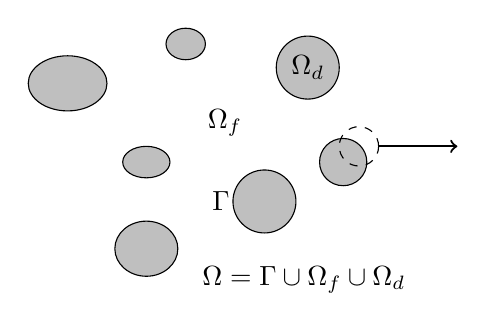
\begin{tikzpicture}
        \foreach \x/\y/\ra/\r in {
        1/3/0.2/0.25,
        2.55/2.7/0.4/0.4,
        0.5/0.4/0.35/0.4,
        2/1/0.4/0.4,
        3/1.5/0.3/0.3,
        0.5/1.5/0.2/0.3,
        -0.5/2.5/0.35/0.5}{
            \draw[fill=gray!50](\x,\y) ellipse(\r cm and \ra cm);
        }
        \draw[dashed](3.2,1.7)circle(0.25);
\draw[thick,->](3.2,1.7)++(0.25,0)--++(1,0);
        \draw(2.55,2.7)node{$\Omega_d$};
        \draw(1.5,2)node{$\Omega_f$};
        \draw(1.45,1)node{$\Gamma$};
        \draw(2.5,0)node{$\Omega = \Gamma \cup \Omega_f \cup \Omega_d$};
\end{tikzpicture}
    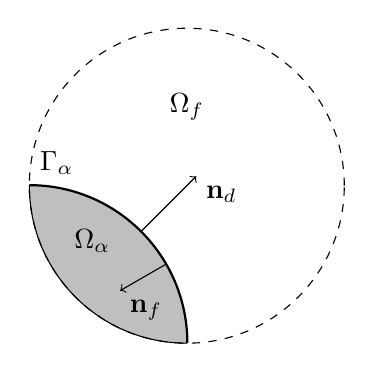
\begin{tikzpicture}\draw[very thick](0:2)arc(0:90:2)node[above right]{$\Gamma_\alpha$};
        \draw[fill=gray!50](0:2)arc(0:90:2)arc(180:270:2);
        \draw[dashed](2,2)circle(2);
        \draw[->](1.42,1.42)--++(0.7,0.7)node[below right]{$\textbf{n}_d$};
        \draw[->](1.73,1)--++(-0.577,-0.333)node[below right]{$\textbf{n}_f$};
        \draw(2,3)node{$\Omega_f$};
        \draw(0.8,1.3)node{$\Omega_\alpha$};
    \end{tikzpicture}
    \caption{Topology of dispersed two-phase flows.}\label{fig:Scheme}
\end{figure}

We consider a system consisting of two phases, separated by a sharp interface $\Gamma(t,\FF)$,
where $t$ represents the current time and $\FF$ a flow realization. Further explanation about the concept of a flow realization will be provided later. 
The phase subdomains are labeled as $\Omega_f(t,\FF)$ and $\Omega_d(t,\FF)$, corresponding to the continuous (fluid) phase ($f$) and the dispersed phase ($d$), respectively (see \DIFdelbegin \DIFdel{Figure }\DIFdelend \ref{fig:Scheme}). 
The complete domain, $\Omega$, is composed of the union of $\Omega_f$, $\Omega_d$, and $\Gamma$. To track the position of phase $k$ and the interfaces, we introduce the phase indicator function $\chi_k$ defined as follows

\begin{align}
    \chi_k(\textbf{x},t,\FF) =  \left\{
      \begin{tabular}{cc}
        $1 \;\text{if} \;\textbf{x} \in \Omega_k(t,\FF)$\\
        $0 \;\text{if} \;\textbf{x} \notin \Omega_k(t,\FF)$
      \end{tabular}
      \right.
      \text{for $k = f,d$}.
      \label{eq:PIF}
\end{align}
Additionally, we define $\Omega_\alpha(t, \FF)$ as the region occupied by particle $\alpha$ at time $t$ within the configuration $\FF$ (\ref{fig:Scheme}). The collective union of $\Omega_\alpha(t, \FF)$ for $\alpha = 1, \ldots, N$, where $N$ denotes the number of particles present in the flow, corresponds to $\Omega_d(t, \FF)$. Similarly, we assume that $\Gamma(t, \FF)$ can be partitioned into $N$ subregions, labeled $\Gamma_\alpha(t, \FF)$, each representing the surface of particle $\alpha$.



\subsection{Topological equations}
Using the distribution formalism, one may show that $\chi_k(\textbf{x},t,\FF)$ obeys the following relations \citep{drew1983mathematical}. 
\begin{align}
    \pddt \chi_k
    + \textbf{u}_\Gamma^0 \cdot \grad \chi_k
    &= 0,
    \label{eq:dt_chi_k}\\
    \label{eq:grad_chi_k}
    \grad \chi_k
    &= - \delta_\Gamma \textbf{n}_k, 
\end{align}
where $\textbf{u}^0_\Gamma(\textbf{x},t,\FF)$ is the velocity of the interface and $\delta_\Gamma(\textbf{x},t,\FF)$ denotes the Dirac function localized \DIFdelbegin \DIFdel{for }\DIFdelend \DIFaddbegin \DIFadd{on }\DIFaddend the interface, also called the interfacial indicator function \citep{drew1983mathematical,junqua2003}. 
More specifically the distribution $\delta_\Gamma$ is defined as \citep{appel2007}
\begin{equation}
<\delta_\Gamma,\phi> =\int_{\Gamma} \phi d\Gamma 
\DIFaddbegin \label{eq:def_surf_distribution}
\DIFaddend \end{equation}  
where $\phi$ is a function with compact support. In this work, we use the subscript $_\Gamma$ to denote any quantity inherently defined on the interfaces, such as $\textbf{u}_\Gamma^0(\textbf{x}, t, \FF)$ and $\delta_\Gamma(\textbf{x}, t, \FF)$. Additionally, we employ the superscript $^0$ on a field to indicate that it is defined at the local, non-averaged level, meaning it is a function of the flow configuration $\FF$, the position vector $\textbf{x}$, and time $t$. For clarity and readability, we omit the arguments $\FF$, $\textbf{x}$, and $t$ for any local function denoted by $^0$ (as well as for $\delta_\Gamma$ and $\chi_k$), as their dependence on $\textbf{x}$, $t$, and $\FF$ is implied.


To derive a conservation equation for $\delta_\Gamma$, one can take the gradient of \ref{eq:dt_chi_k} and then compute the dot product of the resulting expression with $\textbf{n}_k$. This approach yields the following result \citep{marle1982macroscopic,drew1990,lhuillier2000bilan,junqua2003}


\begin{equation}
    \pddt \delta_\Gamma
    + \div [(\textbf{u}_\Gamma^0\cdot \textbf{n}) \textbf{n}\delta_\Gamma ]
    = (\textbf{u}_\Gamma^0 \cdot \textbf{n})(\div\textbf{n}) \delta_\Gamma ,
    \label{eq:dt_delta_I}
\end{equation} 
where we make use of the relation $\textbf{n}_k\cdot \pddt\textbf{n}_k= \frac{1}{2}\pddt(\textbf{n}_k\cdot \textbf{n}_k) = 0$. 
We did not specify the index of the normal $\textbf{n}$ in \ref{eq:dt_delta_I} to emphasize that this equation is independent of the index $k$. This is because $\textbf{n}$ appears twice in each term of this equation. 
\DIFdelbegin \DIFdel{Consequently}\DIFdelend \DIFaddbegin \DIFadd{Likewise}\DIFaddend , we will omit the index of the normal vector in subsequent discussions unless it is required. Additionally, note that in \ref{eq:dt_delta_I} only the normal component of the surface velocity is present, and the term $\div \textbf{n}$ represents twice the mean curvature of the surface \citep{aris2012vectors}.  A second equation is obtained by taking the gradient of the distribution $\delta_\Gamma $ (\ref{ap:delta_I})\DIFaddbegin \DIFadd{, namely, 
}\DIFaddend \begin{equation}
    \grad\delta_\Gamma  
    =   \grad (\textbf{n} \delta_\Gamma) \cdot \textbf{n}.
    \label{eq:grad_delta_I}
\end{equation}
\ref{eq:grad_delta_I} has been derived straightforwardly, yet it differs from the expression recently obtained by \citet{orlando2023evolution}.  The source of this discrepancy is unclear to the current authors. 
It might be due to differences in their notation, with their operator gradient potentially representing a normal derivative. 
\ref{eq:dt_chi_k}, \ref{eq:grad_chi_k}, \ref{eq:dt_delta_I} and \ref{eq:grad_delta_I}  are commonly referred to as the topological equations of two-phase flows.
These equations describe the spatiotemporal evolution of the interfaces topology.

\subsection{Local conservation equations}
\label{sec:local_eq}
We now introduce the local conservation laws that govern the fluid inside bulk phases (inside $\Omega_d$ and $\Omega_f$) and on the interfaces (on $\Gamma$). 
\DIFdelbegin \DIFdel{We present generic conservation laws within the volumes and at the interfaces. 
}\DIFdelend Let $f_k^0$ denote a volumetric quantity of arbitrary tensorial order defined in $\Omega_k$.
Similarly, let $f_\Gamma^0$ represent an arbitrary surface property defined on $\Gamma$. 
\DIFaddbegin \DIFadd{Notice that $f_\Gamma^0$ can be defined as a volumetric quantity integrated over the thickness of the interfaces \mbox{%DIFAUXCMD
\citet[Chapter 2]{ishii2010thermo}}\hspace{0pt}%DIFAUXCMD
. 
Therefore, if $f_k^0$ has units $[x]$, then $f_I^0$ has the unit $[x.L]$, where $L$ is the unit of a length. 
}\DIFaddend The subscript $_{||}$ is used to denote the projection of a field onto the plane tangential to the surface $\Gamma$. Specifically, for an arbitrary quantity $\textbf{g}$ defined on $\Gamma$, its tangential projection is given by $\textbf{g}_{||} = \bm\delta_{||}\cdot \textbf{g}$ where $\bm\delta_{||} = (\bm\delta-\textbf{nn})$ is a tangential projection operator and $\bm\delta$ is the identity tensor. 
This definition also extends to the gradient operator, where $\gradI= \bm\delta _{||}\cdot \grad$ is referred to as the surface gradient operator. In addition we may define the surface divergence operator as $\gradI \cdot ()= (\bm\delta _{||}\cdot \grad)\cdot()$.



Following the strategy outlined in \citep{ishii2010thermo,bothe2022sharp}, the local conservation equations for $f_k^0$ and $f_\Gamma^0$ can be written as follows,
\begin{align}
    \label{eq:dt_f_k}
    \pddt f_k^0
    +\div \left(
        f_k^0\textbf{u}_k^0
        - \mathbf{\Phi}_k^0
        \right)
    &= 
    s_k^0
    & \text{ in } \Omega_k,&\\
    \pddt f_\Gamma^0 
    + f_\Gamma^0 (\textbf{u}_\Gamma^0 \cdot \textbf{n})(\div \textbf{n})
    +\divI
    (f_\Gamma^0 \textbf{u}_{\Gamma||}^0
        - \mathbf{\Phi}_{\Gamma||}^0 )
    &= 
    s_\Gamma^0
    - \Jump{
       f_k (\textbf{u}_\Gamma^0 - \textbf{u}_k^0)
       + \mathbf{\Phi}_k^0
    } 
    & \text{ on } \Gamma.&
    \label{eq:dt_f_I}
\end{align}
The tensors $\mathbf{\Phi}_k^0$ and $\mathbf{\Phi}_{\Gamma||}^0$ represent the non-convective fluxes corresponding to the quantities $f_k^0$ and $f_\Gamma^0$, respectively. Similarly, $s_k^0$ and $s_\Gamma^0$ are the source terms corresponding to the quantities $f_k^0$ and $f_\Gamma^0$, respectively. We assume that only the tangential component of the tensor $\mathbf{\Phi}_{\Gamma}^0$ plays a role in the surface balance equation \citep{bothe2022sharp}. However, in certain specific scenarios, such as momentum transport along a membrane, the interface may exhibit resistance to bending. For further discussion on this topic, see \citet{jaensson2021}. Consequently, the flux terms of the form $\divI[(\ldots)_{||}]$ in \ref{eq:dt_f_I} represent two-dimensional  convective and non-convective fluxes arising from tangential motions or diffusive processes at the interface.
Conversely, the term involving the local curvature $(\div \textbf{n})$ is related to the interface expansion or contraction resulting from the normal velocity of the interface $\textbf{u}_\Gamma^0\cdot \textbf{n}$. For practical uses, note that the advecting term in \ref{eq:dt_f_I} can be written in the more compact form $\divI(f_\Gamma^0 \textbf{u}_\Gamma^0)$. 
Indeed, one can show that $f_\Gamma^0 (\textbf{u}_\Gamma^0 \cdot \textbf{n})(\div \textbf{n})
+\divI(f_\Gamma^0 \textbf{u}_{I||}^0) = \divI(f_\Gamma^0 \textbf{u}_\Gamma^0)$, by noticing that $\textbf{n}\cdot\gradI(\ldots) = 0$ and $\divI\textbf{n} = \div\textbf{n}$ \citep{nadim1996concise}.
In \ref{eq:dt_f_I} we have introduced the notation $\Jump{\ldots}$, where $\Jump{\ldots} = \sum_{k=1}^2 [\ldots] \cdot \textbf{n}_k$ signifies the jump across the interface. Thus, the last term on the right-hand side of \ref{eq:dt_f_I} represent a source of $f_\Gamma^0$ due to the discontinuity of bulk properties on either side of the interface. We also recognize a term related to mass transfer proportional to $(\textbf{u}_\Gamma - \textbf{u}_k)$. It is important to note that \ref{eq:dt_f_k} and \ref{eq:dt_f_I} are uniquely defined within the domains $\Omega_k$ and $\Gamma$, respectively.
Consequently, these equations are referred to as local conservation equations.



 


\subsection{The two-fluid formulation}
The \DIFdelbegin \DIFdel{presence }\DIFdelend \DIFaddbegin \DIFadd{phase indicator }\DIFaddend function $\chi_k$, and the Dirac delta function $\delta_\Gamma $, allow the extension of \ref{eq:dt_f_k} and \ref{eq:dt_f_I} to the entire flow domain $\Omega$. 
This extension is achieved by employing the methodology introduced by \citet{drew1983mathematical} and \citet{kataoka1986local} for the conserving laws inside the volume (\ref{eq:dt_f_k}).
The two-fluid formulation may be obtained by multiplying \ref{eq:dt_f_k} by $\chi_k$. 
Using \ref{eq:dt_chi_k} and \ref{eq:grad_chi_k} we obtain
\begin{equation}
    \pddt (\chi_k f_k^0)
    + \div (
        \chi_k f_k^0 \textbf{u}_k^0
        - \chi_k \mathbf{\Phi}_k^0 
        )
    = 
    \chi_k s_k^0
    + \delta_\Gamma \left[
        f_k^0
        \left(
            \textbf{u}_\Gamma^0
            - \textbf{u}_k^0
        \right)
        + \mathbf{\Phi}_k^0
    \right]
    \cdot \textbf{n}_k.
    \label{eq:dt_chi_k_f_k}
\end{equation}
This yields an equation defined over $\Omega$, to be solved for the quantity $\chi_k f_k^0$ instead of $f_k^0$. 
Moreover, in contrast to \ref{eq:dt_f_k} we observe the emergence of the interfacial term $ \delta_\Gamma [\ldots]$ on the right-hand side of \ref{eq:dt_chi_k_f_k}. 
To the best of the author's knowledge, the general form of the interfacial transport equation, expressed using the distribution formalism, has not yet been derived. However, some specific forms applicable to a given $f_i$ can be found in \citet{marle1982macroscopic} and  \citet{teigen2009}.
The derivation of this equation is straightforward but requires some algebra which is detailed in \ref{ap:interface_proof}. This yields\begin{equation}
    \pddt (\delta_\Gamma f_\Gamma^0)  
    + \div (
        \delta_\Gamma  f_\Gamma^0 \textbf{u}_\Gamma^0
        - \delta_\Gamma  \mathbf{\Phi}_{\Gamma||}^0 
        )
    = 
    \delta_\Gamma s_\Gamma^0
    - \delta_\Gamma \Jump{
    f_k^0 (\textbf{u}_\Gamma^0 - \textbf{u}_k^0)
    + \mathbf{\Phi}_k^0},
    \label{eq:dt_delta_I_f_I}
\end{equation}
which corresponds to the conservation equation of $\delta_\Gamma f_\Gamma^0$, which is defined over $\Omega$.
Although \ref{eq:dt_f_I} and \ref{eq:dt_delta_I_f_I} appear similar in many respects, they possess a fundamental distinction: \ref{eq:dt_f_I} is defined exclusively on $\Gamma$, it is a two-dimensional partial differential equation with a time-dependent metric, whereas \ref{eq:dt_delta_I_f_I} is a three-dimensional partial differential equation. 
This distinction holds significant importance, as the formulation of \ref{eq:dt_delta_I_f_I} proves to be more practical for the numerical modeling of quantities on deformable interfaces \citep{teigen2009}. The set of equations formed by \ref{eq:dt_chi_k_f_k} for $k = f,d$ and the surface transport equation or \textit{jump condition} (\ref{eq:dt_delta_I_f_I}) is commonly known as the \textit{two-fluid} formulation of multiphase flows \citep{morel2015mathematical,tryggvason2011direct,drew1983mathematical,kataoka1986local}. 

\DIFdelbegin \DIFdel{Let us }\DIFdelend \DIFaddbegin \DIFadd{According to \ref{eq:def_surf_distribution} the distribution  $\delta_\Gamma$ has the dimension of the inverse of a length, $[L^{-1}]$ \mbox{%DIFAUXCMD
\citep{appel2007}}\hspace{0pt}%DIFAUXCMD
. 
Thus, assuming that $f_k^0$ has the dimension of $[x]$, implies that $f_\Gamma^0$ is of dimension $[x.L]$, and therefore also means that the product $\delta_\Gamma f_\Gamma^0$ is of unit $[x]$.
Consequently, we }\DIFaddend define a \textit{bulk} property $f^0$ as $f^0 = \sum_{k} \chi_k f_k^0 + \delta_\Gamma  f_\Gamma^0$ where $f^0$ represents any property of the flow of arbitrary tensorial order.
Then by summing \ref{eq:dt_chi_k_f_k} for $k=f,d$ and \ref{eq:dt_delta_I_f_I}, one obtain the \textit{bulk} formulation of multiphase flows, namely,\begin{equation}
   \pddt f^0
   + \div (
       \mathbf{F}^0
       -  \mathbf{\Phi}^0 
    )
   = s^0. 
   \label{eq:dt_f}
\end{equation}
where $\mathbf{F}^0 = \sum_{k} \chi_k \mathbf{f}_k^0\textbf{u}_k^0 + \delta_\Gamma  \mathbf{f}_\Gamma^0\textbf{u}_\Gamma^0$, $\mathbf{\Phi}^0 = \sum_{k} \chi_k \mathbf{\Phi}_k^0 + \delta_\Gamma  \mathbf{\Phi}_\Gamma^0$ and $s^0 = \sum_{k} \chi_k s_k^0 + \delta_\Gamma  s_\Gamma^0$. 
In the literature, the \textit{single-fluid} formulation is characterized by summing only the quantities within the two phases, while the interfacial components are treated as source terms \citep{tryggvason2011direct,morel2015mathematical}.
Nevertheless, we want to point out here that our definition of $f^0$ yields a straightforward transport equation for $f^0$ thereby ensuring the consistency of the entire system of equations.



 \subsection{The averaged conservation equations}
\label{sec:avg_def}
In this study, we employ the ensemble average technique to establish the averaged conservation equations. 
This method is just one of several averaging approaches, including the volume average method \citep{jackson1997locally} and time averaging \citep{ishii2010thermo}. 
Although these techniques differ, they ultimately produce the same set of averaged equations, as evidenced by comparing volume averaging theory with ensemble averaging theory \citep{jackson1997locally,zhang1997momentum}. However, for slightly non-uniform suspensions, ensemble averaging is better suited for deriving the averaged equations because it does not require assumptions about the characteristic length scale of the spatial filter \citep{lhuillier1992ensemble}.
In the following we recall some properties of the ensemble average operator. 
Let, $P(\FF)$ be the probability density function that describes the probability of finding the flow in the configuration $\FF$. 
We note $d\PP = P(\FF) d\FF$ the probable number of flows located in the incremental region of the phase space $d\FF$ around the point $\FF$. 
It follows from this definition, that the ensemble average of an arbitrary local property $f^0(\textbf{x},t;\FF)$ defined on the whole space $\Omega$, is,
\begin{equation}
    f(\textbf{x},t)
    = \avg{f^0}(\textbf{x},t)
    =\int f^0(\textbf{x},t;\FF) d\mathscr{P}. 
    \label{eq:avg}
\end{equation}  
Note that we dropped the super script $^0$ on $f(\textbf{x},t)$ to indicate that this is an averaged quantity. 
The macroscopic variables are averaged over all $\FF$, and therefore depend only on $\textbf{x}$ and $t$.
Thus, we omit the arguments of the averaged fields, as this notation eliminates any potential ambiguity. 
The ensemble average quantities are assumed to satisfy the following properties \citep{drew1983mathematical}
\begin{align}
    \avg{f^0+h^0} = f+h, 
    && \avg{\avg{f^0}h^0} = fh, \nonumber\\
    \avg{\pddt f^0} 
    = \pddt f,  
    &&\avg{\grad f^0}
    = \grad f. 
    \label{eq:avg_properties}
\end{align}
were $f$ and $h$ are two arbitrary Eulerian fields. 
The first two relations are called the Reynolds' rules, the third one is the Leibniz' rule and the last one, is the Gauss' rule \citep{drew1983mathematical}.
Additionally, for any phase quantity defined in $\Omega_k$ we introduce the definition, 
\begin{equation}
    \phi_k f_k (\textbf{x},t) = \avg{\chi_k f_k^0},
    \label{eq:1_avg}
\end{equation}
where $\phi_k(\textbf{x},t) = \avg{\chi_k}$ is the probability of finding the phase $k$ at the location \textbf{x} and time $t$.
And $f_k$ is the average of the field $f_k^0$ conditioned on the presence of the phase $k$ in the configuration $\FF$ at $\textbf{x}$ and time $t$.
Equally, for interface quantities we have 
\begin{equation}
    \phi_\Gamma f_\Gamma (\textbf{x},t) = \avg{\delta_\Gamma f_\Gamma^0},
\end{equation}
with $\phi_\Gamma = \avg{\delta_\Gamma}$ the probability of finding the interface at the point \textbf{x} at time $t$. 
Here, $f_\Gamma$ is the average of $f^0_\Gamma$ conditioned on the presence of an interface in the configuration $\FF$ at $\textbf{x}$ and time $t$. 
Additionally, we define the field of fluctuation of a given quantity around its mean as,
\begin{align}
    f'(\textbf{x},t,\FF) = f^0(\textbf{x},t,\FF) - f(\textbf{x},t).
    \label{eq:def_fluctu}
\end{align}
This relation applies to phase averaged quantities such that $f'_k = f^0_k - f_k$ and $f'_\Gamma = f^0_\Gamma - f_\Gamma$. 


Applying the ensemble average on \ref{eq:dt_chi_k_f_k} and \ref{eq:dt_delta_I_f_I} and considering the properties from \ref{eq:avg_properties} to \ref{eq:def_fluctu}, yields the general form of the averaged equations of multiphase flows, namely,
\begin{align}
    \pddt (\phi_k f_k)
    +\div (\phi_k f_k \textbf{u}_k + \mathbf{\Phi}_k^\text{eq})
    &= 
    \phi_k s_k
    + \avg{\delta_\Gamma\left[
        \mathbf{\Phi}_k^0
        + f_k^0
        \left(
            \textbf{u}_\Gamma^0
            - \textbf{u}_k^0
        \right)
    \right]
    \cdot \textbf{n}_k},
    \label{eq:avg_dt_chi_f}\\
    \pddt (\phi_\Gamma f_\Gamma)
    +\div (\phi_\Gamma f_\Gamma \textbf{u}_\Gamma+ \mathbf{\Phi}_\Gamma^\text{eq})
    &= 
    \phi_\Gamma s_\Gamma
    - \avg{\delta_\Gamma 
    \Jump{
    \mathbf{\Phi}_k^0
    + f_k^0 (\textbf{u}_\Gamma^0 - \textbf{u}_k^0)
    } 
     },
    \label{eq:avg_dt_delta_f}
\end{align}
with, 
\begin{align}
    \mathbf{\Phi}_k^\text{eq}
    = \avg{\chi_k f_k' \textbf{u}_k'}
    - \phi_k \bm\Phi_k,
    &&
    \mathbf{\Phi}_\Gamma^\text{eq}
    = \avg{\delta_\Gamma f_\Gamma' \textbf{u}_\Gamma'}
    - \phi_\Gamma \bm\Phi_\Gamma. 
\end{align}
These equations are to be solved for the averaged field \DIFdelbegin \DIFdel{$\phi_k,\phi_\Gamma,f_k$ }\DIFdelend \DIFaddbegin \DIFadd{$f_f,f_d$, }\DIFaddend and $f_\Gamma$\DIFdelbegin \DIFdel{with a complementary equation of volume conservation, i.
e. $\phi_f+\phi_d+\phi_\Gamma = 1$}\DIFdelend .
The main differences between these equations and their microscale counterparts (\ref{eq:dt_f_k} and \ref{eq:dt_f_I}) are:
(1) The unknowns are now averaged quantities,
(2) \DIFdelbegin \DIFdel{Factors }\DIFdelend \DIFaddbegin \DIFadd{factors }\DIFaddend $\phi_k$ and $\phi_\Gamma$ are introduced in front of all the terms, and
(3) \DIFdelbegin \DIFdel{The }\DIFdelend \DIFaddbegin \DIFadd{the }\DIFaddend additional terms $\avg{\chi_k f_k' \textbf{u}_k'}$ and $\avg{\delta_\Gamma f_\Gamma' \textbf{u}_\Gamma'}$ appear, representing the covariance between the conserved quantity ($f_k$ or $f_\Gamma$) and the local velocities.  



It is important to highlight that the two-fluid model fails to adequately distinguish between the two phases, as evidenced by the \textit{symmetry} $k = 1$ and $2$ in the aforementioned equations. This symmetry does not hold physically because the dispersed phase possesses a distinct topological nature compared to the continuous phase. 
In a dispersed two-phase flow system, the closure terms are typically expressed as functions of the Lagrangian properties of the particles \citep{jackson2000}. In contrast, the current system of equations yields continuously averaged quantities, which are not directly connected to the Lagrangian properties.
Therefore, in the subsequent section, we will introduce a \DIFdelbegin \DIFdel{kinetic based }\DIFdelend \DIFaddbegin \DIFadd{kinetic-based }\DIFaddend model specifically devoted to the dispersed phase. 
As illustrated below, the equations governing the dispersed phase are more comprehensive as they bear a resemblance to the equations governing a single particle.

 

\section{Lagrangian equations for the dispersed phase}
\label{sec:Lagrangian}

Lagrangian-based modeling of the dispersed phase has been explored extensively in numerous studies \citep{buyevich1979flow, lhuillier1992volume, simonin1996, zhang1994averaged, zhang1994ensemble, zhang1997momentum, jackson1997locally, zaepffel2011modelisation}. However, these studies predominantly focus on solid particles \citep{buyevich1979flow, lhuillier1992volume, simonin1996, zhang1994averaged, jackson1997locally} or non-deformable spherical fluid inclusions \citep{zhang1994ensemble, zaepffel2011modelisation}. A notable exception is the work by \citep{zhang1994ensemble}, which considered spherical bubbles with varying radii, although this analysis was limited to constant surface tension and spherical shapes. In this work, we aim to address a more general scenario by considering fluid particles with arbitrary shapes and surface properties. Thus, we propose a Lagrangian-based model for each inclusion capable of describing the dispersed phase with arbitrary accuracy. 

 \subsection{Fundamental properties of the dispersed phase}
We define the mass $m_\alpha$, the position of center of mass $\mathbf{x}_\alpha$ and the momentum $\textbf{p}_\alpha$ as
\begin{align}
    m_\alpha(t,\FF)
    &= \DIFdelbegin %DIFDELCMD < \intO{ \rho_d  }%%%
\DIFdelend \DIFaddbegin \intOF{ \rho_d  }\DIFaddend , 
    \\
    \textbf{x}_\alpha(t,\FF)
    &= \frac{1}{m_\alpha }\DIFdelbegin %DIFDELCMD < \intO{ \rho_d \textbf{x} }     %%%
\DIFdelend \DIFaddbegin \intOF{ \rho_d \textbf{x} }     \DIFaddend \label{eq:mass_pos0},
    \\ \textbf{p}_\alpha(t,\FF)
    &= \DIFdelbegin %DIFDELCMD < \intO{ \rho_d \textbf{u}_d^0 }%%%
\DIFdelend \DIFaddbegin \intOF{ \rho_d \textbf{u}_d^0 }\DIFaddend .
\end{align}
Note that while the mass of the interface might be considered in the center of mass calculation, in practice, the mass within the volume is typically much greater than the mass on the interface. 
Therefore, we have opted to use the more straightforward definition considering only the mass within the particle volume.
Subsequently, we define the velocity of the particle center of mass as
\begin{equation}
\textbf{u}_\alpha(t,\FF) = \frac{d \textbf{x}_\alpha}{dt}.
\label{eq:u_alpha}
\end{equation}
We also define the particle's internal relative motions or the \textit{inner velocity}  as $\textbf{w}_d^0 = \textbf{u}_d^0 - \textbf{u}_\alpha$. 
Similarly we define $\textbf{w}_I^0$ as $\textbf{w}_I^0 = \textbf{u}_{I||}^0 - \textbf{u}_\alpha$.
Replacing $\textbf{x}_\alpha$ by its definition (\ref{eq:mass_pos0}) in \ref{eq:u_alpha} we obtain
\begin{equation}
    \textbf{u}_\alpha(t,\FF) = \frac{1}{m_\alpha}
    \frac{d}{dt} 
    \left(
        \DIFdelbegin %DIFDELCMD < \intO{ \rho_d \textbf{x} }
%DIFDELCMD <     %%%
\DIFdelend \DIFaddbegin \intOF{ \rho_d \textbf{x} }
    \DIFaddend \right)
    - \frac{1}{m_\alpha^2} \frac{d}{dt} \left(\DIFdelbegin %DIFDELCMD < \intO{ \rho_d } %%%
\DIFdelend \DIFaddbegin \intOF{ \rho_d } \DIFaddend \right)
    \DIFdelbegin %DIFDELCMD < \intO{ \rho_d \textbf{x} }%%%
\DIFdelend \DIFaddbegin \intOF{ \rho_d \textbf{x} }\DIFaddend .
\end{equation}
Using \ref{eq:reynolds_transport} for both terms in parentheses and the definition of $\textbf{x}_\alpha(t,\FF)$ in the last term gives
\begin{align}
    \textbf{u}_\alpha(t,\FF) &=  \frac{1}{m_\alpha}\DIFdelbegin %DIFDELCMD < \intO{
%DIFDELCMD <         \pddt (\textbf{x}\rho_d ) + \div\left(\textbf{u}_d^0 \textbf{x} \rho_d\right) 
%DIFDELCMD <     } 
%DIFDELCMD <     %%%
\DIFdelend \DIFaddbegin \intOF{
        \pddt (\textbf{x}\rho_d ) + \div\left(\textbf{u}_d^0 \textbf{x} \rho_d\right) 
    } 
    \DIFaddend + \frac{1}{m_\alpha}\DIFdelbegin %DIFDELCMD < \intS{ \textbf{x} \rho_d(\textbf{u}_I - \textbf{u}_d^0) \cdot \textbf{n}_d } %%%
\DIFdelend \DIFaddbegin \intSF{ \textbf{x} \rho_d(\textbf{u}_I - \textbf{u}_d^0) \cdot \textbf{n}_d } \DIFaddend \nonumber\\
    & - \frac{1}{m_\alpha^2}\DIFdelbegin %DIFDELCMD < \intO{
%DIFDELCMD <         \pddt (\rho_d ) + \div\left(\textbf{u}_d^0 \rho_d\right) 
%DIFDELCMD <     } %%%
\DIFdelend \DIFaddbegin \intOF{
        \pddt (\rho_d ) + \div\left(\textbf{u}_d^0 \rho_d\right) 
    } \DIFaddend -  \frac{\textbf{x}_\alpha}{m_\alpha}    \DIFdelbegin %DIFDELCMD < \intS{ \rho_d(\textbf{u}_I   - \textbf{u}_d^0) \cdot \textbf{n}_d }
%DIFDELCMD <     \label{eq:u_alpha}
%DIFDELCMD < %%%
\DIFdelend \DIFaddbegin \intSF{ \rho_d(\textbf{u}_I   - \textbf{u}_d^0) \cdot \textbf{n}_d }
    \label{eq:u_alpha2}
\DIFaddend \end{align}
Making use of the conservation of mass\DIFdelbegin \DIFdel{the firt }\DIFdelend \DIFaddbegin \DIFadd{, the first }\DIFaddend term on the second line of \DIFdelbegin \DIFdel{\ref{eq:u_alpha} }\DIFdelend \DIFaddbegin \DIFadd{\ref{eq:u_alpha2} }\DIFaddend vanishes. This yields,\DIFdelbegin \begin{displaymath}
    \DIFdel{\textbf{u}_\alpha(t,\FF) = 
    \frac{1}{m_\alpha}\intO{ \left[
        \pddt (\textbf{x}\rho_d ) + \div\left(\textbf{u}_d^0 \textbf{x} \rho_d\right) 
    \right]} }\\
    \DIFdel{+ \frac{1}{m_\alpha}\intS{ \textbf{x} \rho_d(\textbf{u}_\Gamma^0   - \textbf{u}_d^0) \cdot \textbf{n}_d }
    -  \frac{\textbf{x}_\alpha}{m_\alpha}    \intS{ \rho_d(\textbf{u}_\Gamma^0   - \textbf{u}_d^0) \cdot \textbf{n}_d }
}\end{displaymath}%DIFAUXCMD
\DIFdelend \DIFaddbegin \begin{multline}
    \DIFadd{\textbf{u}_\alpha(t,\FF) = 
    \frac{1}{m_\alpha}\intOF{ \left[
        \pddt (\textbf{x}\rho_d ) + \div\left(\textbf{u}_d^0 \textbf{x} \rho_d\right) 
    \right]} }\\
    \DIFadd{+ \frac{1}{m_\alpha}\intSF{ \textbf{x} \rho_d(\textbf{u}_\Gamma^0   - \textbf{u}_d^0) \cdot \textbf{n}_d }
    -  \frac{\textbf{x}_\alpha}{m_\alpha}    \intSF{ \rho_d(\textbf{u}_\Gamma^0   - \textbf{u}_d^0) \cdot \textbf{n}_d }
}\end{multline}\DIFaddend 
Then by considering the mass conservation for the first term and noticing that $\grad \textbf{x} = \bm\delta$ gives\begin{equation}
    \textbf{u}_\alpha(t,\FF) = \frac{1}{m_\alpha(t,\FF)} \left(
        \textbf{p}_\alpha(t,\FF)
        +  \DIFdelbegin %DIFDELCMD < \intS{\rho_d \textbf{r} (\textbf{u}_\Gamma^0 - \textbf{u}_d^0)\cdot \textbf{n}_d }
%DIFDELCMD <         %%%
\DIFdelend \DIFaddbegin \intSF{\rho_d \textbf{r} (\textbf{u}_\Gamma^0 - \textbf{u}_d^0)\cdot \textbf{n}_d }
        \DIFaddend \right),
        \label{eq:dt_y_alpha}
\end{equation}
where $\textbf{r}(\textbf{x},t,\FF) = \textbf{x} - \textbf{x}_\alpha(t,\FF)$ is the distance between any point inside $\Omega_\alpha$, to the center of mass of the particle $\alpha$.
In \ref{eq:dt_y_alpha}, it can be observed that the first component of the velocity represents the linear momentum divided by the mass of the particle. 
This corresponds to the mass-averaged velocity over the volume of the particle.
The second term in \ref{eq:dt_y_alpha} arises from the contribution of anisotropic mass transfer across the surface of the particle. 
This mass transfer leads to the motion of the particle's center of mass, thereby contributing to the total velocity.
To illustrate this concept, let us consider a fixed drop with no momentum lying over a very hot plate.
In this scenario, we assume that the plate is sufficiently hot to induce evaporation, specifically on the bottom portion of the drop.
Hence, under the effect of an anisotropic evaporation flux one may expect the second term to be non-negligible.
Consequently, the center of mass of the drop has a non-zero velocity in the opposite direction of the plate, even though the momentum is assumed to be zero.
Note that \ref{eq:dt_y_alpha} generalized usual expression of the center of mass velocity whom neglect the second term.
In the following, for the sake of brevity we discard the dependency on $t$ and $\FF$ on the notations for all Lagrangian quantities denoted by the subscript $_\alpha$ and in particular $\Gamma_\alpha$ and $\Omega_\alpha$.
Nevertheless, the reader must understand that all Lagrangian quantities and integration domains subscribed by $_\alpha$ are time and configuration-dependent. 



\subsection{Lagrangian conservation laws}




We assign to a particle indexed, $\alpha$, occupying the domain $\Omega_\alpha$ (see \ref{fig:Scheme}) an arbitrary Lagrangian property $\text q_\alpha$ defined by $\text q_\alpha  = \intO{ f_d^0}$. The Reynolds transport theorem for the (material) particle volume can be written as \citep{leal2007advanced},


\begin{equation}
\ddt  \intO{f_d^0}
    = \intO{\pddt f_d^0 }\\
    + \intS{ f_d^0 \textbf{u}_\Gamma^0\cdot \textbf{n}_d }.
    \label{eq:reynolds_transport0}
\end{equation}
\DIFdelbegin \DIFdel{Using the divergence theorem the last equation may be rewritten as
}\DIFdelend \DIFaddbegin \DIFadd{Adding and subtracting $f_d^0 \textbf{u}_d^0\cdot \textbf{n}_d$ in the last integral of this equation and using the divergence theorem, yields
}\DIFaddend \begin{equation}
    \ddt  \intO{f_d^0}
    = \intO{\left[ \pddt f_d^0 + \div\left(f_d^0\textbf{u}_d^0\right) \right]}\\
    + \intS{ f_d^0 (\textbf{u}_\Gamma^0-\textbf{u}_d^0)\cdot \textbf{n}_d }.
    \label{eq:reynolds_transport}
\end{equation}
By substituting \ref{eq:dt_f_k} into \ref{eq:reynolds_transport} and using the divergence theorem we obtain the conservation law of the quantity $\text q_\alpha$ \begin{equation}
    \frac{d \text q_\alpha}{d t}
    = \intO{ s_d^0 }
    + \intS{ \left[
        f_d^0 (\textbf{u}_\Gamma^0-\textbf{u}_d^0) 
        + \mathbf{\Phi}_d^0 
        \right] \cdot \textbf{n}_d }.
    \label{eq:dt_q_alpha}
\end{equation}
The first term on the right-hand side of \ref{eq:dt_q_alpha} accounts for the total contribution of the source term $s_d^0$ to the particle $\alpha$,
while the second term is the surface integration of the phase exhange flux $f_d^0 (\textbf{u}_\Gamma^0-\textbf{u}_d^0)$ and the non-convective flux $\mathbf{\Phi}_d^0$.

Similarly, we define $\text q_{\Gamma\alpha} = \intS{ f_\Gamma^0}$ as an integrated surface property of the particle $\alpha$.
To differentiate time-varying surface integrals with respect to time, we make use of the surface Reynolds transport theorem, which reads \citep[Appendix B]{morel2015mathematical} \begin{equation}
    \ddt  \intS{f_\Gamma^0 }
    = \intS{ \left[
        \frac{D_\Gamma f_\Gamma^0}{Dt}+
        +   f_\Gamma^0\gradI \cdot \textbf{u}_\Gamma^0
    \right]}.
    \label{eq:surface_derivative}
\end{equation}
where $\frac{D_\Gamma}{Dt}  = \pddt + \textbf{u}_\Gamma^0\cdot \gradI $ is the material derivative operator on the surface of the particle. 
Upon expanding the acceleration term we obtain the expression,
\begin{equation}
    \ddt  \intS{f_\Gamma^0 }
    = \intS{ \left[
        \pddt f_\Gamma^0
        +   \gradI \cdot (\textbf{u}_\Gamma^0f_\Gamma^0)
    \right]}.
    \label{eq:surface_derivative}
\end{equation}
Then inserting \ref{eq:dt_f_I} into \ref{eq:surface_derivative} we obtain
\begin{equation}
    \ddt  \text q_{\Gamma\alpha}
    = \intS{ 
        \gradI \cdot \boldsymbol{\Phi}_{\Gamma||}^0
    }
    +\intS{ 
        s_\Gamma^0
    }
    - \intS{
 \Jump{
        f_k^0 (\textbf{u}_\Gamma^0 - \textbf{u}_k^0)
        + \mathbf{\Phi}_k^0
    }
    }.
    \label{eq:dt_q_I_alpha}
\end{equation}
The surface divergence theorem applied to closed surfaces  reads \citep{nadim1996concise}
\begin{equation}
    \intS{\gradI F}
    = 
    \intS{ F \cdot\textbf{n} (\div \textbf{n})},
    \label{eq:gauss_surface}
\end{equation} 
where $F$ is an arbitrary field.
This theorem demonstrates that any surface property parallel to the tangential plane of $\Gamma$, such as $\bm\Phi_{I||}$, fulfills the condition $\intS{\divI \bm\Phi_{I||}^0}
= 0$.
\DIFdelbegin \DIFdel{This }\DIFdelend \DIFaddbegin \DIFadd{Therefore \ref{eq:dt_q_I_alpha} }\DIFaddend yields,

\begin{equation}
    \ddt  \text q_{\Gamma\alpha}
    = \intS{ 
        s_\Gamma^0
    }
    - \intS{
 \Jump{
        f_k^0 (\textbf{u}_\Gamma^0 - \textbf{u}_k^0)
        + \mathbf{\Phi}_k^0
    }
    }.
    \label{eq:dt_q_I_alpha}
\end{equation}
In \ref{eq:dt_q_alpha}, the non-convective flux within the dispersed phase appears on the right hand side. While this is not problematic for fluid particles for which the internal stress is defined, the stress within rigid particles is not defined \citep{batchelor1970stress}.
Hence to remove the internal stress from \ref{eq:dt_q_alpha}, we treat the particle's volume and surface as a single entity and derive a conservation equation for $\text Q_\alpha = \text q_\alpha + \text q_{\Gamma\alpha}$. 
By summing \ref{eq:dt_q_alpha} and \ref{eq:dt_q_I_alpha} we directly obtain 
\begin{equation}
    \ddt  \text Q_\alpha
    = 
    \intO{ s_d^0 }
    + \intS{ s_\Gamma^0 }
    + \intS{ \left[
        f_f^0 (\textbf{u}_\Gamma^0-\textbf{u}_f^0) 
        + \mathbf{\Phi}_f^0 
        \right] \cdot \textbf{n}_d }. 
    \label{eq:dt_q_alpha_tot}
\end{equation}
This equation is the general form of the linear conservation law for the quantity $\text Q_\alpha$.
It applies to any particle immersed in a continuous phase following the conservation laws given by \ref{eq:dt_f_k} and \ref{eq:dt_f_I}.
We refer to this equation as the zeroth-order conservation equation \DIFaddbegin \DIFadd{of $f_d^0$}\DIFaddend , or alternatively, the linear conservation law \DIFaddbegin \DIFadd{of $f_d^0$, }\DIFaddend for the particle $\alpha$.
We would like to highlight that due to the consideration of closed surface, the non-convective flux $\mathbf{\Phi}_{\Gamma||}^0$, does not appear in \ref{eq:dt_q_alpha_tot}.
Consequently, for the conservation of linear momentum, the surface stresses does not contribute to the momentum balance of a particle.
As a result, surface tension or surface viscous stresses do not directly affect the linear momentum balance \footnote{However, Marangoni effect can induce motion through the imbalance of tangential stress \citep{young1959}. Indeed the resulting imbalance alters the stress within the continuous phase, generating a hydrodynamic force.}. 
This property has already been demonstrated by \citet{hesla1993note} who showed that the surface tension force does not contribute to the linear and angular momentum balance. 
Here, we have provided the general proof that the interfacial non-convective flux $\mathbf{\Phi}_{\Gamma||}^0$, which is present at the local scale according to \ref{eq:dt_f_I}, does not contribute to the zeroth-order conservation law of a particle with a closed surface.
It is important to note that this conclusion is valid only if the non-convective flux is parallel to the interface, which is what we assumed here.









\subsection{Higher order moment equations}


Because $f_d^0$ and $f_\Gamma^0$ are not always constant over the volumes and surfaces of the particles, it is interesting to introduce the first moment of the quantities $f_d^0$ and $f_\Gamma^0$. 
They are defined as $\textbf{q}_\alpha^{(1)}     = \intO{ \textbf{r} f_d^0 }$ and $\textbf{q}_{\Gamma\alpha}^{(1)}    = \intS{ \textbf{r} f_\Gamma^0 }$.  
In general, the first moments $\textbf{q}^{(1)}_{\alpha}$ and $\textbf{q}^{(1)}_{\Gamma\alpha}$ hold significant importance when considering particles with high internal gradients, i.e. when $\grad f_d^0$ or $\gradI f_\Gamma^0$ are non-negligible at the scale of one particle. 
Typically, when considering the motion of a fiber, one must consider the angular momentum balance \citep{guazzelli2011}, which corresponds to the antisymmetric part of the first moment of momentum.
It is possible to differentiate the moments $\textbf{q}^{(1)}_\alpha$ and $\textbf{q}^{(1)}_{\Gamma\alpha}$  with respect to time to obtain their conservation laws.
We use \ref{eq:reynolds_transport} to describe the evolution of $\textbf{q}^{(1)}_\alpha$ within time. This yields, 
\begin{equation}
    \frac{d}{dt} \textbf{q}^{(1)}_\alpha
      =  \intO{\left[
        \pddt(  f_d^0\textbf{r})
        + \div \left(  f_d^0 \textbf{r}\textbf{u}_d^0\right)
    \right]} 
    + \intS{  f_d^0 \textbf{r}  (\textbf{u}_\Gamma^0-\textbf{u}_d^0)\cdot \textbf{n}_d}.
\end{equation}
The first term on the right-hand side may be rewritten as
\begin{equation}
\intO{ \left[
        \pddt(\textbf{r}  f_d^0)+ \div \left( \textbf{u}_d^0 \textbf{r} f^0_d\right) 
    \right]}
    = \intO{\textbf{r}\left[
        \pddt f_d^0
        + \div \left(f_d^0 \textbf{u}_d^0\right)
    \right] }
    + \intO{ f_d^0 \left[
        \pddt \textbf{r}
        +(\textbf{u}_d^0 \cdot \grad) \textbf{r}
    \right]}
\end{equation}
Substituting \ref{eq:dt_f_k} in the first integral on the right-hand side, and considering the relation,
$  \pddt \textbf{r}
+ (\textbf{u}_d^0 \cdot \grad) \textbf{r}
= - \frac{d}{dt} \textbf{x}_\alpha  + \textbf{u}_d^0 
= \textbf{w}_d^0$,
for the second integral yields 
\begin{align}
    \frac{d}{dt} \textbf{q}^{(1)}_\alpha = \intO{\textbf{r} (s_d^0 +\div \bm\Phi_d^0)  }
    + \intO{ f_d^0\textbf{w}_d^0 }  + \intS{  f_d^0 \textbf{r}  (\textbf{u}_\Gamma^0-\textbf{u}_d^0)\cdot \textbf{n}_d}
\end{align}
Then using relation $\intO{\textbf{r}  \div \bm\Phi_d^0 }
= \intS{ \textbf{r} \bm\Phi_d^0 \cdot \textbf{n}_d }
- \intO{ \bm\Phi_d^0 }$ we get
\begin{align}
    \frac{d}{dt} \textbf{q}^{(1)}_\alpha
= \intO{\left( 
        \textbf{r} s_d^0  
        + f_d^0  \textbf{w}_d^0
        - \bm\Phi_d^0
    \right) }
    + \int_{\Gamma_\alpha} \textbf{r} \left[
        \bm\Phi_d^0
        + f_d^0 (\textbf{u}_\Gamma^0-\textbf{u}_d^0)
    \right]\cdot \textbf{n}_d  d\Sigma.
    \label{eq:dt_Q_alpha}
\end{align}
 \ref{eq:dt_Q_alpha} is the first order moment conservation equation for the particle $\alpha$. 
 In \ref{eq:dt_Q_alpha}, we recognize the first moment of the source term $s_d^0$, the first moment of the non convective flux term $\bm\Phi_d^0\cdot\textbf{n}_d$ and the first moment of phase exchange term, $f_d^0 (\textbf{u}_\Gamma^0-\textbf{u}_d^0)\cdot\textbf{n}_d$. 
 Additionally, two supplementary terms appear in \ref{eq:dt_Q_alpha}, namely: the volume integral of the non convective flux $\bm\Phi_d^0$, and a term related to the fluctuation of the internal velocity $f_d^0 \textbf{w}_d^0$.

Following the same procedure, and making use of \ref{eq:dt_f_I}, \ref{eq:surface_derivative} and \ref{eq:gauss_surface} , one can equally show that 
\begin{align}
    \ddt {\textbf{q}^{(1)}_{\Gamma\alpha}}
    &= \intS{ \left(
        \textbf{r}s_\Gamma^0
        + f_\Gamma^0 \textbf{w}_\Gamma^0
        - \mathbf{\Phi}_{||\Gamma}^0
    \right) }
    - \intS{\textbf{r} 
    \Jump{\mathbf{\Phi}_k^0
        + f_k^0 (\textbf{u}_\Gamma^0 - \textbf{u}_k^0)
    }
    },
    \label{eq:dt_Q_I_alpha}
\end{align}
Observations similar to those for \ref{eq:dt_Q_alpha} can also be made for the first moment of surface equation \ref{eq:dt_Q_I_alpha}.
In particular, it is worth noting the presence of the surface non-convective flux $\mathbf{\Phi}_{\Gamma||}^0$ in \ref{eq:dt_Q_I_alpha}.


For similar reason than the linear conservation equations, we sum \ref{eq:dt_Q_alpha} and \ref{eq:dt_Q_I_alpha} to express the conservation equation of the total first moment $\textbf{Q}^{(1)}_\alpha = \textbf{q}^{(1)}_\alpha + \textbf{q}^{(1)}_{\Gamma\alpha}$, this yields 
\begin{multline}
    \ddt {\textbf{Q}^{(1)}_\alpha}
    = \intO{ \left(
        \textbf{r} s_d^0         
        + f_d^0  \textbf{w}_d^0 
        - \mathbf{\Phi}_d^0
    \right) }
    + \intS{ \left(
        \textbf{r}s_\Gamma^0
        + f_\Gamma^0 \textbf{w}_\Gamma^0
        - \mathbf{\Phi}_{\Gamma||}^0
    \right) }
    + \intS{ \textbf{r} \left[
        \mathbf{\Phi}_f^0
        + f_f^0 (\textbf{u}_\Gamma^0-\textbf{u}_f^0)
    \right]\cdot \textbf{n}_d  }. 
    \label{eq:dt_Q_alpha_tot}
\end{multline}
Likewise, conservation laws can be derived for the $n^{th}$ order moments of volume and surface, i.e. for
\begin{align}
    \textbf{q}^{(n)}_{\alpha}
    = \intO{
         \underbrace{\textbf{rr}\ldots \textbf{rr}}_{n\text{ times}}
        f_d^0 },
        && \text{and} &&
    \textbf{q}\DIFdelbegin \DIFdel{^{(1)}}\DIFdelend \DIFaddbegin \DIFadd{^{(n)}}\DIFaddend _{\Gamma\alpha}
    = \intS{
         \underbrace{\textbf{rr}\ldots \textbf{rr}}_{n\text{ times}}
    f_\Gamma^0 },
    \label{eq:Q_n_definition}
\end{align} 
respectively. The time derivatives of $\textbf{q}^{(n)}_{\alpha}$ and $\textbf{q}^{(n)}_{\Gamma\alpha}$ do not introduce any additional terms beyond those already present in equations \ref{eq:dt_Q_alpha} and \ref{eq:dt_Q_I_alpha}.
Instead, they only involve the $n^{th}$ order moments of the existing terms.
We provide the full derivation of $\ddt{ \textbf{q}^{(n)}_{\alpha}}$ in \ref{ap:Moments_equations}.
The higher-order moments characterize the distributions of the local quantities $f_d^0$ and $f_\Gamma^0$ within the regions $\Omega_\alpha$ and $\Gamma_\alpha$​, respectively. 
To precisely reconstruct the fields $f_d^0$ and $f_\Gamma^0$ within $\Omega_\alpha$ and $\Gamma_\alpha$​, an infinite number of moments would theoretically be required. 
\DIFaddbegin \DIFadd{Nevertheless, as pointed out by \mbox{%DIFAUXCMD
\citet[Appendix A]{zhang1997momentum}}\hspace{0pt}%DIFAUXCMD
, when the degrees of freedom of the particles are limited (solid particles, spherical droplets in stokes flows\ldots), only a finite number of moments are necessary to reconstruct $f_d^0$ and $f_\Gamma^0$. 
}\DIFaddend 


 

\section{Hybrid description of the two phases}
\label{sec:averaged_eq}

Two distinct descriptions can be applied to the dispersed phase, while only one description is applicable to the \DIFdelbegin \DIFdel{fluid }\DIFdelend \DIFaddbegin \DIFadd{continuous }\DIFaddend phase. 
In this section, we derive averaged equations for the dispersed phase using Lagrangian conservation laws. 
Following this, we  discuss the equivalence between the particle or Lagrangian averaged equations for the dispersed phase and the averaged equations for the dispersed phase presented in \ref{sec:two-fluid}.




\subsection{Particle-averaged equations}

In the preceding section, we have described the dispersed phase using a Lagrangian framework. 
However, to ensure consistency with the Eulerian conservation equations that describe the continuous phase, it is necessary to extend the Lagrangian equations to an Eulerian description. 
The approach presented here follows the methodology pioneered by \citep{lhuillier1992ensemble}.
We introduce the function $\delta_\alpha$, which is defined as follows, 
\begin{align}
    \delta_\alpha(\textbf{x},\textbf{x}_\alpha(t,\FF)) 
    = \delta(\textbf{x}-\textbf{x}_\alpha(t,\FF)),
    \label{eq:delta_alpha}
\end{align}
where $\delta$ is the Dirac function.
Note that we explicitly note the arguments $(t,\FF)$ to highlight that the position of the particle $\alpha$ is a function of time and of the flow configuration $\FF$.
\DIFdelbegin \DIFdel{Applying the }\DIFdelend \DIFaddbegin \DIFadd{Taking the time derivative on $\delta_\alpha$ and 
applying the }\DIFaddend chain rule yields \citep{lhuillier1998}\begin{equation}
    \pddt \delta_\alpha
    + \div (\textbf{u}_\alpha  \delta_\alpha)
    =0,
    \label{eq:dt_delta_alpha}
\end{equation}
where we used the identity, $\frac{\partial \delta_\alpha}{\partial \textbf{x}_\alpha}  = -\grad \delta_\alpha$ and the fact that $\textbf{u}_\alpha(t,\FF)$ is not a function of $\textbf{x}$. 
\ref{eq:dt_delta_alpha} does not apply in scenarios where topological changes occur, such as break-up or coalescence events. 
In these cases, a source term can be introduced on the right-hand side of \ref{eq:dt_delta_alpha}, similar to the approach used in population balance equations, to account for the birth or death of particles \citep{randolph2012theory}.
Consider a domain containing $N$ particles. We define the \textit{particle field} for a quantity $\text q_\alpha$​ as the sum of $\delta_\alpha \text q_\alpha$ over all particles within the domain, expressed by $\displaystyle\sum_{\alpha=0}^N \delta_\alpha \text q_\alpha$​. 
Note that the formula given by \DIFdelbegin \DIFdel{\ref{eq:dt_delta_alpha_q_alpha} }\DIFdelend \DIFaddbegin \DIFadd{\ref{eq:dt_delta_alpha} }\DIFaddend remains valid for the sum of such fields, since the operations of differentiation and summation commute.
To obtain the averaged equations for the dispersed phase, we define the particle average of $\text q_\alpha$​ as
\begin{equation}
     n_p \text q_p(\textbf{x},t) = \avg{\sum_\alpha\delta_\alpha \text q_\alpha},
     \label{eq:p_avg}
\end{equation}
where, $n_p(\textbf{x},t) = \avg{\sum_\alpha \delta_\alpha}$ is the probability density of finding a particle center of mass in the infinitesimal volume $d\textbf{x}$ around \textbf{x}, and $\text q_p(\textbf{x},t)$ is the average of $\text q_\alpha$ conditionally on the presence of a particle\DIFaddbegin \DIFadd{'s center of mass }\DIFaddend at \textbf{x} and time $t$. 
To simplify the notations, we consider the shorthand \citep{lhuillier1998},
\begin{equation*}
    \sum_\alpha \delta_\alpha \to \delta_p, 
\end{equation*}
such that $\pavg{\text q_\alpha}=\avg{\sum_\alpha \delta_\alpha \text q_\alpha}=n_p\text q_p$.
Note that we used the subscript $_p$ on $\text q_p$ to denote that this represents a particle-averaged field, initially derived from Lagrangian quantities. 
Additionally, in light of \ref{eq:def_fluctu} we define the fluctuating part of a particle field $\text q_p$ as
\begin{equation}
    \text q_\alpha'\DIFaddbegin \DIFadd{(}\textbf{\DIFadd{x}}\DIFadd{,t,}\FF\DIFadd{) }\DIFaddend = \text q_\alpha\DIFaddbegin \DIFadd{(}\FF\DIFadd{,t) }\DIFaddend - \text q_p\DIFaddbegin \DIFadd{(}\textbf{\DIFadd{x}}\DIFadd{,t)}\DIFaddend . 
    \label{eq:def_fluc_p}
\end{equation}

To derive the averaged equations for the particle phase, we begin by noting that multiplying a Lagrangian quantity $\text q_\alpha$​ by $\delta_\alpha$​ yields the corresponding Eulerian field  $\text q_\alpha(t,\FF)\delta_\alpha(\textbf{x},t,\FF)$, which is defined throughout the entire domain $\Omega$. 
Similarly, for any derivative of a Lagrangian quantity, such as $\ddt \text q_\alpha$​, the corresponding Eulerian field is defined by multiplying $\ddt \text q_\alpha$ with $\delta_\alpha$.
Given that $\text q_\alpha(t,\FF)$ and $\textbf{u}_\alpha(t,\FF)$ do not depend on \textbf{x}, and by using Equation \ref{eq:dt_delta_alpha}, we obtain
\begin{equation}
    \delta_\alpha \ddt \text q_\alpha
    = \pddt (\delta_\alpha \text q_\alpha)
    + \div (\delta_\alpha \text q_\alpha \textbf{u}_\alpha).
    \label{eq:dt_delta_alpha_q_alpha}
\end{equation}
Multiplying \ref{eq:dt_q_alpha_tot} and \ref{eq:dt_Q_alpha_tot} by $\delta_\alpha$, using \ref{eq:dt_delta_alpha_q_alpha} and applying the ensemble average (\ref{eq:avg}), yields
\begin{align}
    \pddt (n_p\text Q_p)
    + \div (n_p \text Q_p \textbf{u}_p + \pavg{\textbf{u}_\alpha' \text Q_\alpha'})
    = \pOavg{ s_d^0 }
    + \pSavg{ s_I^0 }\nonumber\\
    + \pSavg{ \left[\mathbf{\Phi}_f^0 + f_f^0 (\textbf{u}_\Gamma^0-\textbf{u}_f^0) \right] \cdot \textbf{n}_d },
    \label{eq:avg_dt_dq_alpha_tot}\\
    \pddt (n_p\textbf{Q}_p^{(1)})
    + \div \left(n_p \textbf{Q}_p^{(1)} \textbf{u}_p + \pavg{\textbf{u}_\alpha' \textbf{Q}_\alpha^{(1)'}}\right)
    =\pOavg{ \left(
        \textbf{r} s_d^0         
        + f_d^0  \textbf{w}_d^0 
        - \mathbf{\Phi}_d^0
    \right) }\nonumber\\
    + \pSavg{ \left(
        \textbf{r}s_\Gamma^0
        + f_\Gamma^0 \textbf{w}_\Gamma^0
        - \mathbf{\Phi}_{\Gamma||}^0
    \right) }
    + \pSavg{ \textbf{r} \left[
        \mathbf{\Phi}_f^0
        + f_f^0 (\textbf{u}_\Gamma^0-\textbf{u}_f^0)
    \right]\cdot \textbf{n}_d  }.
    \label{eq:avg_dt_dQ_alpha_tot}
\end{align}
The derivation of the higher moment particle-averaged equations is provided in \ref{ap:Moments_equations}.
The only fluxes appearing in \ref{eq:avg_dt_dq_alpha_tot} and \ref{eq:avg_dt_dQ_alpha_tot} are the fluctuation tensors $\pavg{\textbf{u}_\alpha' \text q_\alpha'}$ and $\pavg{\textbf{u}_\alpha' \textbf{Q}_\alpha'}$. 
Therefore, the non-convective fluxes $\bm\Phi_d^0$ and $\bm\Phi_I^0$ do not play the role of macroscopic fluxes, as it is the case in \ref{eq:avg_dt_chi_f} and \ref{eq:avg_dt_delta_f}. Instead, they act as source terms in the first moment and higher moment equations. 
This distinction is the main structural differences between the Kinetic-like model (\ref{eq:avg_dt_dq_alpha_tot} and \ref{eq:avg_dt_dQ_alpha_tot}) and the two-phase flow model (\ref{eq:avg_dt_chi_f} and \ref{eq:avg_dt_delta_f}). 
In this study, \ref{eq:avg_dt_chi_f} and \ref{eq:avg_dt_delta_f} are referred to as the phase-averaged equations, while \ref{eq:avg_dt_dq_alpha_tot} and \ref{eq:avg_dt_dQ_alpha_tot} are called the particle-averaged equations. 


 



 
\subsection{Equivalence between particle-averaged and phase-averaged equations}
\label{sec:equivalence}
To model the dispersed phase, there are two distinct approaches. 
We can either use \ref{eq:avg_dt_chi_f} with $k=d$, or we can employ the particle-averaged equations \ref{eq:avg_dt_dq_alpha_tot}, \ref{eq:avg_dt_dQ_alpha_tot} and potentially the higher moments equations found in \ref{ap:Moments_equations}.
Consequently, it is important to address the compatibility between these two formalisms.
It has been demonstrated in various studies \citep{buyevich1979flow,lhuillier1992ensemble,jackson1997locally,zhang1994averaged}, that phase-averaged quantities can be expressed as a Taylor series expansion of particle-averaged quantities. 
\DIFdelbegin %DIFDELCMD < \tb{
%DIFDELCMD < Indeed, the dispersed phase indicator function $\chi_d$ can be expressed as a sum of phase indicator function, $\chi_d(\textbf{x},t,\FF) = \sum_\alpha\chi_\alpha(\textbf{x},t,\FF)$ where $\chi_\alpha =1$ in the particle domain $\Omega_\alpha(\FF,t)$ and $0$ otherwise. 
%DIFDELCMD < Thus, any dispersed phase quantity can be written as, 
%DIFDELCMD < \begin{displaymath}
%DIFDELCMD <    f^0_d \chi_d(\textbf{x},t,\FF)
%DIFDELCMD <    = \sum_\alpha f^0_d \chi_\alpha(\textbf{x},t,\FF) 
%DIFDELCMD < = 
%DIFDELCMD <    \sum_\alpha 
%DIFDELCMD <    \int_{\mathbb{R}^3} 
%DIFDELCMD <     f^0_d \chi_\alpha(\textbf{x},t,\FF)\delta(\textbf{x}_\alpha(\FF,t) - \textbf{y}) 
%DIFDELCMD <     d\textbf{y} 
%DIFDELCMD <    \label{eq:taylor_f_d}
%DIFDELCMD < \end{displaymath}
%DIFDELCMD < Where we have noticed that, 
%DIFDELCMD < \begin{displaymath}
%DIFDELCMD <     \int_{\mathbb{R}^3}\delta(\textbf{x}_\alpha(\FF,t) - \textbf{y}) d\textbf{y} = 1. 
%DIFDELCMD < \end{displaymath}
%DIFDELCMD < Additionally, in the integral on the left-hand side of \ref{eq:taylor_f_d}, notice that $\textbf{x} = \textbf{x}_\alpha + \textbf{r}$ with $\textbf{r} = (\textbf{x} - \textbf{x}_\alpha) = \textbf{x} - \textbf{y}$,
%DIFDELCMD < where replaced $\textbf{x}_\alpha$ by \textbf{y} in the last identity since the Dirac delta function reduce the integration on the configurations where $\textbf{x}_\alpha = \textbf{y}$.
%DIFDELCMD < Thus, without approximation we write, 
%DIFDELCMD < \begin{displaymath}
%DIFDELCMD <     f^0_d \chi_d(\textbf{x},t,\FF) = 
%DIFDELCMD <     \sum_\alpha 
%DIFDELCMD <     \int_{\mathbb{R}^3} 
%DIFDELCMD <      f^0_d \chi_\alpha(\textbf{x}_\alpha + \textbf{r},t,\FF)\delta(\textbf{x}_\alpha(\FF,t) - \textbf{y}) 
%DIFDELCMD <      d\textbf{y} 
%DIFDELCMD <     \label{eq:f_d_reform}
%DIFDELCMD < \end{displaymath}
%DIFDELCMD < Likewise, we assume that the interface indicator function $\delta_\Gamma$ can be partitioned into $N$ interface indicator function such that $\delta_\Gamma = 
%DIFDELCMD < \sum_\alpha  \delta_{\Gamma\alpha}$.
%DIFDELCMD < In that case any surface-averaged quantities may be written, 
%DIFDELCMD < \begin{displaymath}
%DIFDELCMD <     f_\Gamma^0 \delta_\Gamma(\textbf{x},t,\FF) = 
%DIFDELCMD <     \sum_\alpha 
%DIFDELCMD <     \int_{\mathbb{R}^3} 
%DIFDELCMD <      f_\Gamma^0 \delta_{\Gamma\alpha}(\textbf{x}_\alpha + \textbf{r},t,\FF)\delta(\textbf{x}_\alpha(\FF,t) - \textbf{y}) 
%DIFDELCMD <      d\textbf{y}. 
%DIFDELCMD <     \label{eq:f_G_reform}
%DIFDELCMD < \end{displaymath}
%DIFDELCMD < Notice that the product of the two distribution is allowed since $\delta_{\Gamma\alpha}$ is evaluated according to the variable $\textbf{x}$, while $\delta(\textbf{x}_\alpha - \textbf{y})$ has its singularity at the point \textbf{y}. 
%DIFDELCMD < Upon using the Taylor expansion of the Dirac delta function $\delta(\textbf{x}_\alpha - \textbf{y}) = \delta(\textbf{x}_\alpha - \textbf{x}- \textbf{r})$ in the neighborhood of $\textbf{r}=0$ one obtain
%DIFDELCMD < \begin{displaymath}
%DIFDELCMD < \delta(\textbf{x}_\alpha - \textbf{x}-\textbf{r}) 
%DIFDELCMD < = \delta(\textbf{x}_\alpha - \textbf{x}) 
%DIFDELCMD < - \textbf{r}\cdot\grad \delta(\textbf{x}_\alpha - \textbf{x}) 
%DIFDELCMD < + \frac{\textbf{rr}}{2}:\grad\grad\delta(\textbf{x}_\alpha- \textbf{x}) - \ldots.
%DIFDELCMD < \label{eq:exp_delta}
%DIFDELCMD < \end{displaymath}
%DIFDELCMD < Injecting \ref{eq:exp_delta} into \ref{eq:f_d_reform} and \ref{eq:f_G_reform}, and noticing that the indicator functions, $\chi_\alpha$ and $\delta_\Gamma$, reduce the domain of integration to, $\Omega_\alpha$ and $\Gamma_\alpha$, respectively,  gives, 
%DIFDELCMD < \begin{eqnarray*}
%DIFDELCMD <     f^0_d \chi_d(\textbf{x},t)
%DIFDELCMD <     =\delta_p\intO{f^0_d}
%DIFDELCMD <     - \div\left(\delta_p\intO{\textbf{r} f^0_d}\right)
%DIFDELCMD <     + \frac{1}{2}\grad\grad :\left(\delta_p\intO{\textbf{rr} f^0_d}\right)
%DIFDELCMD <     \ldots 
%DIFDELCMD <     \label{eq:fd_asympt}
%DIFDELCMD <    \\
%DIFDELCMD <    f_\Gamma^0 \delta_\Gamma (\textbf{x},t)
%DIFDELCMD <    =\delta_p\intS{f^0_\Gamma}
%DIFDELCMD <    - \div\left(\delta_p\intS{\textbf{r} f^0_\Gamma}\right)
%DIFDELCMD <    + \frac{1}{2}\grad\grad :\left(\delta_p\intS{\textbf{rr} f^0_\Gamma}\right)
%DIFDELCMD <    \ldots 
%DIFDELCMD <    \label{eq:fG_asympt}
%DIFDELCMD < \end{eqnarray*}
%DIFDELCMD < respectively. 
%DIFDELCMD < Where we recognize the zeroth, first and second order moments of $f_d^0$ and $f_\Gamma^0$, into \ref{eq:fd_asympt} and \ref{eq:fG_asympt}, respectively. 
%DIFDELCMD < Notice that even before applying any kind of averaging procedure \ref{eq:fd_asympt} and \ref{eq:fG_asympt} illustrates the connection between the dispersed phase fields, of the form $\chi_d(\ldots)$ or $\delta_\Gamma(\ldots)$ , and the particle fields of the form $\delta_p(\ldots)$. 
%DIFDELCMD < It is interesting to notice that this relation hols even if it may seem counterintuitive. 
%DIFDELCMD < }
%DIFDELCMD < %%%
\DIFdel{Averaging \ref{eq:fd_asympt} and \ref{eq:fG_asympt} }\DIFdelend \DIFaddbegin \DIFadd{Applying similar considerations to the interface indicator function $\delta_\Gamma$, and averaging }\DIFaddend over all configurations, we obtain the general relations that link continuous-averaged and particle-averaged fields, namely \citep{lhuillier1992ensemble,lhuillier1998,lhuillier2000bilan}, 
\begin{align}
    \avg{\chi_df_d^0} 
    &=  \pavg{\text q_\alpha}
        - \div  
        \pavg{\textbf{q}_\alpha^{(1)}}        
        + \frac{1}{2} \grad\grad : \pavg{\textbf{q}_{\alpha}^{(2)}}
        + \ldots  \label{eq:f_exp_chi} \\
    \avg{\delta_\Gamma  f_\Gamma ^0} 
    &=  \pavg{\text q_{\Gamma \alpha}}        
        - \div \pavg{\textbf{q}_{\Gamma\alpha}^{(1)}}
        + \frac{1}{2} \grad\grad : \pavg{\textbf{q}_{\Gamma\alpha}^{(2)}}
        + \ldots  
    \label{eq:f_exp_delta}
\end{align}
Summing \ref{eq:f_exp_chi} and \ref{eq:f_exp_delta} we obtain
\begin{equation}
    \avg{\chi_df_d^0+\delta_\Gamma  f_\Gamma ^0} = \pavg{\text Q_\alpha}
    - \div  
    \pavg{\textbf{Q}_\alpha^{(1)}}        
    + \frac{1}{2} \grad\grad : \pavg{\textbf{Q}_{\alpha}^{(2)}}
    + \ldots  \label{eq:f_exp}
\end{equation}
When considering an infinite number of terms in \ref{eq:f_exp} one might eventually obtain a converged approximation of \DIFdelbegin \DIFdel{$\chi_d f_d^0+\delta_\Gamma  f_\Gamma ^0$}\DIFdelend \DIFaddbegin \DIFadd{$\avg{\chi_d f_d^0+\delta_\Gamma  f_\Gamma ^0}$}\DIFaddend . 
However, it is important to note that Taylor series have what is known as a \textit{radius of convergence} beyond which adding more terms does not necessarily improve the approximation \citep[Chapter 1]{appel2007}. 
In particular, for distances beyond a certain limit \textbf{r} the series might diverges depending on the behavior of the function $\avg{\chi_d f_d^0+\delta_\Gamma  f_\Gamma ^0}$ near the point \DIFdelbegin \DIFdel{$\textbf{x}_\alpha$}\DIFdelend \DIFaddbegin \DIFadd{$\textbf{x}$}\DIFaddend . 
For the purposes of this article, we will assume that the Taylor series has an infinite radius of convergence, although this assumption warrants further investigation.





To demonstrate the equivalence between the two formalisms, we follow a strategy similar to \citep{lhuillier2000bilan,lhuillier2009rheology}. 
Let $\mathcal{C}_d$ denote the phase-averaged equation of conservation (\ref{eq:avg_dt_chi_f} with $k=d$) and $\mathcal{C}_\Gamma $ the averaged surface transport equation (\ref{eq:avg_dt_delta_f}).
Specifically, they are defined as follows
\begin{align}
    \mathcal{C}_d
    &=
    - \pddt \avg{\chi_df_d^0}
    - \div \avg{\chi_d \mathbf{\Phi}_d^0 - \chi_df_d^0 \textbf{u}_d^0}
    + \avg{\chi_d s_d^0}
    + \avg{\delta_\Gamma \left[
        \mathbf{\Phi}_d^0
        + f_d^0
        \left(
            \textbf{u}_\Gamma ^0
            - \textbf{u}_d^0
        \right)
    \right]
    \cdot \textbf{n}_d},\\
    \mathcal{C}_\Gamma 
    &= 
    -\pddt \avg{\delta_\Gamma f_\Gamma ^0}
    -\div \avg{\delta_\Gamma  f_\Gamma ^0 \textbf{u}_\Gamma ^0-\delta_\Gamma  \mathbf{\Phi}_{I||}^0 }
    + \avg{\delta_\Gamma s_\Gamma ^0} 
    - \avg{\delta_\Gamma  \Jump{
     \mathbf{\Phi}_k^0+
    f_k^0 (\textbf{u}_\Gamma ^0 - \textbf{u}_k^0)
    } }. 
\end{align}
It should be noted from \ref{eq:avg_dt_chi_f} and \ref{eq:avg_dt_delta_f} that $\mathcal{C}_d\equiv 0$ and $\mathcal{C}_\Gamma  \equiv 0$.
By applying the Taylor expansion to each term of $\mathcal{C}_d+\mathcal{C}_\Gamma $ as described in \ref{eq:f_exp} yields
\begin{equation}
    \mathcal{C}_d 
    + \mathcal{C}_\Gamma  
    = \mathcal{M}^{(0)} - \div \mathcal{M}^{(1)} + \frac{1}{2} \grad\grad : \mathcal{M}^{(2)} \ldots = 0,
    \label{eq:scheme_equivalence}
\end{equation} 
where the expressions for $\mathcal{M}^{(0)}$ and $\mathcal{M}^{(1)}$ are given by 
\begin{align}
    &\mathcal{M}^{(0)}
    = 
    - \avg{\delta_p \ddt {\text Q_\alpha}}
+ \pOavg{ s_d^0 }
    + \pSavg{ s_\Gamma ^0 }
    + \pSavg{ 
    \left[\mathbf{\Phi}_f^0 
    + f_f^0 (\textbf{u}_\Gamma ^0-\textbf{u}_f^0) \right] \cdot \textbf{n}_d },\\
    &\mathcal{M}^{(1)} =
    -  \avg{\delta_p \ddt {\textbf{Q}_\alpha^{(1)}}}
+ \pOavg{ \left(
        \textbf{r} s_d^0         
        + f_d^0  \textbf{w}_d^0 
        - \mathbf{\Phi}_d^0
    \right) }
    + \pSavg{ \left(
        \textbf{r}s_\Gamma ^0
        + f_\Gamma ^0 \textbf{w}_\Gamma ^0
        - \mathbf{\Phi}_{\Gamma||}^0
    \right) } \nonumber\\
    &+ \pSavg{ \textbf{r} \left[
        \mathbf{\Phi}_f^0
        + f_f^0 (\textbf{u}_\Gamma ^0-\textbf{u}_f^0)
    \right]\cdot \textbf{n}_d  }.
\end{align}
Using \ref{eq:scheme_equivalence}, we reach one of the main conclusion of this study. 
We observe that $\mathcal{M}^{(0)}$ and $\mathcal{M}^{(1)}$ correspond to the zeroth and first-order moment equations, respectively. 
Additionally, as demonstrated in \ref{ap:Moments_equations} the coefficient $\mathcal{M}^{(n)}$ in \ref{eq:scheme_equivalence} represents the $n^{th}$ order moment in the particle-averaged conservation equation. 
From \ref{eq:scheme_equivalence} we conclude that combining \ref{eq:avg_dt_chi_f} for $k=d$ and \ref{eq:avg_dt_delta_f} effectively captures the particle moment equations through a Taylor expansion around the particle center of mass. 
Therefore, it is clear that by considering an arbitrary order of particle moments equations, one can achieve a highly accurate description of the dispersed phase.


The particle-averaged equations ($\mathcal{M}^{(0)}$\ldots $\mathcal{M}^{(n)}$) form a system with $n$ equations, one for each moment. 
In contrast, the \DIFaddbegin \DIFadd{dispersed }\DIFaddend phase-averaged equations ($\mathcal{C}_d$ \DIFdelbegin \DIFdel{and }\DIFdelend \DIFaddbegin \DIFadd{+ }\DIFaddend $\mathcal{C}_\Gamma$) consist of only two equations, which aggregate all the particle-averaged equations. 
This indicates that the particle-averaged formalism provides more \DIFdelbegin \DIFdel{detailed }\DIFdelend information since it yields a separate equation for each moment, as opposed to the phase-averaged equations, which are limited to just two. 
This enhanced level of detail is achieved by considering the topology of the dispersed phase as demonstrated in the previous sections.












\subsection{Conservation equations}

Given that the aim of this work is not only to demonstrate the equivalence but also to establish a comprehensive framework for analyzing dispersed two-phase flows, we now present \textit{the hybrid} set of conservation equations.
The system of equations governing a macroscopic quantity $f$ consists of one equation for the fluid phase, which ensures the conservation of $f_f$ and $n$ equations for the dispersed phase, representing the conservation of the quantities $\textbf{Q}_p^{(n)}$.  
In its most general form, the hybrid description of $f$ can be expressed as
\begin{align}
    \pddt (\phi_f f_f)
    +\div (\phi_f f_f \textbf{u}_f \DIFdelbegin \DIFdel{- }\DIFdelend \DIFaddbegin \DIFadd{+ }\DIFaddend \mathbf{\Phi}_f^\text{eff})
    &= 
    \phi_f s_f
    - \pSavg{\left[
        \mathbf{\Phi}_f^0
        + f_f^0
        \left(
            \textbf{u}_\Gamma^0
            - \textbf{u}_f^0
        \right)
    \right]
    \cdot \textbf{n}_d} ,
    \label{eq:avg_hybrid_dt_chi_f}\\
\pddt (n_p\text Q_p)
        + \div (n_p \text Q_p \textbf{u}_p + \pavg{\textbf{u}_\alpha' \text Q_\alpha'})
        &= \pOavg{ s_d^0 }
        + \pSavg{ s_\Gamma^0 }\nonumber\\
        &+ \pSavg{ \left[\mathbf{\Phi}_f^0 + f_f^0 (\textbf{u}_\Gamma^0-\textbf{u}_f^0) \right] \cdot \textbf{n}_d },
        \label{eq:avg_hybrid_q}
        \\
        \pddt (n_p\textbf{Q}_p^{(1)})
        + \div (n_p \textbf{Q}_p^{(1)} \textbf{u}_p + \pavg{\textbf{u}_\alpha' (Q_\alpha^{(1)})'})
        &=\pOavg{ \left(
            \textbf{r} s_d^0         
            + f_d^0  \textbf{w}_d^0 
            - \mathbf{\Phi}_d^0
        \right) }\nonumber\\
        + \pSavg{ \left(
            \textbf{r}s_\Gamma^0
            + f_\Gamma^0 \textbf{w}_\Gamma^0
            - \mathbf{\Phi}_{I||}^0
        \right) }
        &+ \pSavg{ \textbf{r} \left[
            \mathbf{\Phi}_f^0
            + f_f^0 (\textbf{u}_\Gamma^0-\textbf{u}_f^0)
        \right]\cdot \textbf{n}_d  },
        \label{eq:avg_hybrid_q_1}
        \\\nonumber
        \vdots
\end{align}
where the effective continuous phase non-convective flux term reads 
\begin{align}
    \mathbf{\Phi}_f^\text{eff}
    = \avg{\chi_f f_f' \textbf{u}_f'}
    - \avg{\chi_f \bm\Phi_f^0}
    - \pSavg{\textbf{r}\left[
        \mathbf{\Phi}_f^0
        + f_f^0
        \left(
            \textbf{u}_\Gamma^0
            - \textbf{u}_f^0
        \right)
    \right]
    \cdot \textbf{n}_d}
    + \div[\ldots].
\end{align}
The only difference in the conservation equation for the continuous phase between \eqref{eq:avg_dt_chi_f} and \eqref{eq:avg_hybrid_dt_chi_f} is the expansion of the exchange term $\avg{\delta_\Gamma \left[
    \mathbf{\Phi}_f^0
    + f_f^0
    \left(
        \textbf{u}_\Gamma ^0
        - \textbf{u}_f^0
    \right)
\right]
\cdot \textbf{n}_d}$ into a Taylor series in a similar way to \ref{eq:f_exp_delta}. 
The presence of the terms $\div[\ldots]$ in the expression for  $\mathbf{\Phi}_f^\text{eff}$ suggests that higher-order moments of the interphase exchange term are involved.
Similarly, the ellipsis below \ref{eq:avg_hybrid_q_1} implies that an arbitrary number of dispersed phase moment equations can be introduced. In this format, it becomes evident that the exchange term on the right-hand side of \ref{eq:avg_hybrid_dt_chi_f} is identical to that on the right-hand side of \ref{eq:avg_hybrid_q}. 
Additionally, in the effective flux $\mathbf{\Phi}_f^\text{eff}$ the exchange term from  \ref{eq:avg_hybrid_q_1} appears, and this property continues for higher-order moments.  
Consequently, the zeroth order exchange term in the equation for $\text Q_\alpha^{(0)}$ plays the role of a source term for $f_f$, while the first and higher order exchange terms act as a source into the higher moment equations, and contribute to the effective non-convective fluxes for $f_f$. 



The system of equations presented here offers a clear understanding of the roles of the dispersed phase non-convective flux terms, $\bm\Phi_d$ and $\bm\Phi_\Gamma$, in the particle phase conservation equation. 
As evidenced in \ref{eq:avg_hybrid_q}, $\bm{\Phi}_d$ and $\bm{\Phi}_\Gamma$  do not influence the lowest order particle-phase averaged conservation equation, i.e. the equation of $n_p \text Q_p$. 
However, \ref{eq:avg_dt_chi_f} (for $k = d$) and \ref{eq:avg_dt_delta_f}, show that the phase-averaged quantities $f_d$ and $f_\Gamma$, are affected by the non-convective fluxes at the particle surface and internally, since $\bm{\Phi}_d$ and $\bm{\Phi}_\Gamma$ appear in these equations.
This may seem contradictory at first, but it is important to note that $\bm{\Phi}_d^0$ and $\bm{\Phi}_\Gamma^0$ serve as source terms in the conservation equations for higher moments such as $\textbf{Q}^{(1)}_p$ \ldots $\textbf{Q}^{(n)}_p$, which are related to $f_d$ and $f_\Gamma$ through \ref{eq:f_exp}.
In summary, the non-convective fluxes $\bm{\Phi}_d$ and $\bm{\Phi}_\Gamma$  are not explicitly related to $\text Q_p$, regardless of particle nature or volume fraction. 
Instead, their influence on $\text Q_p$ is mediated through the closure terms in equation \ref{eq:avg_hybrid_q}, which may depend on the higher moments $\textbf{Q}^{(1)}_p$ \ldots $\textbf{Q}^{(n)}_p$ or other higher-order particle-related moments.These moments, in turn, explicitly depend on $\bm{\Phi}_d$ and $\bm{\Phi}_\Gamma$ as indicated by \ref{eq:avg_hybrid_q_1}. 






 





\section{Discussion}
\label{sec:conclusion}
The system consists of $n+1$ equations for $n+1$ unknowns, specifically $f_f$, $\textbf{Q}_p^{(1)}$\ldots$\textbf{Q}_p^{(n)}$ \footnote{Mote that $\phi_f$ and $n_p$ can also be treated as unknowns by adding corresponding equations, achieved by setting $f_f=1$ and $Q_\alpha^{(n)} =1$ in \ref{eq:avg_hybrid_dt_chi_f} and \ref{eq:avg_hybrid_q}.}.
 The closure problem then involves deriving explicit expressions for all terms of \DIFaddbegin \DIFadd{\ref{eq:avg_hybrid_dt_chi_f} to \ref{eq:avg_hybrid_q_1}, of }\DIFaddend the form $\avg{\ldots}$ in terms of the problem's unknowns, i.e. 
 $f_f$, $\text Q_\alpha$, $\text Q_\alpha^{(1)}$ \ldots $ \text Q_\alpha^{(n)}$.  
 Once these expressions are determined, the equations can be solved. 
 The closure problem presents a great challenge, and has only been addressed in very specific cases. 
 In what follows, we will review the limited attempts made to close the momentum equation in viscous dominated flows. 
 Despite the extensive work on this topic, only a few theoretical results exist that fully account for the whole closure problem. 
 In the regime of Stokes flow and for very dilute suspensions, \citet{jackson1997locally} and \citet{zhang1997momentum} independently derived the momentum closure for spherical solid particles, with \citet{zhang1997momentum} extending the work to spherical drops. 
 The inclusion of the symmetric part of the first moment of momentum, namely the stresslet, leads to Einstein's viscosity formula. 
 Even in this regime, the averaged fluid phase exhibits non-Newtonian behavior, induced by the relative motion of the particles due to the incorporation of quadratic terms in the velocity field far from the particles.
 There have been very few efforts to extend these results to finite Reynolds number regimes. \citet{stone2001inertial} demonstrated that, in the case of general linear flow, the effect of finite inertia is to produce normal stresses, leading to non-Newtonian behavior, while the effective viscosity remains unchanged with respect to Einstein's original formula. 
 This prediction was recently extended to the case of drops by \citet{raja2010inertial}. 
 In a work in preparation we investigate the effects of drop translation at finite Reynolds numbers on the stresslet.






The last question we now aim to address is: in what circumstances is the inclusion of higher moments, such as $\textbf{Q}_p^{(n)}$, necessary within this system of equations?
There are two primary reasons why the moment $\textbf{Q}_p^{(n)}$ may be required:
\begin{itemize}
\item First when $\textbf{Q}_p^{(n)}$ provides critical information sought in the analysis. 
For example, consider the case of fiber orientation in a flow, which corresponds to the second moment of the particle mass distribution. 
This information might be the central objective of the study, especially when the goal is to understand how fiber orientation evolves in industrial applications like composite materials \citep{advani1987use}.

\item Second $\textbf{Q}_p^{(n)}$is essential for accurately modeling closure terms. 
Again, fiber orientation serves as a relevant example. 
Indeed in dilute flows of axisymmetric fibers within the Stokes regime the force acting on the fiber (which represents the closure term in the momentum equation) is dependent on the fiber orientation \citep{kim2013microhydrodynamics}. Another example directly relevant to the focus of this article involves the transport of surfactants. 
Consider a dilute flow of spherical bubbles rising in a liquid contaminated by soluble surfactants. 
When a bubble ascends through the flow, surfactants are transported along the bubble surface, leading to the formation of a stagnant cap on the side opposite to the bubble direction of motion \citep{cuenot1997effects}.
The surfactant uneven concentration field on the interface, gives rise to a spatially variable surface tension coefficient. 
Furthermore, this variation in surface tension induces additional Marangoni stresses. These Marangoni stresses alter the flow around the bubble surface, significantly affecting the drag force experienced by the rising bubble \citep{cuenot1997effects,pesci2018computational}. 
This influence is governed by the surfactant concentration and its distribution, which can be characterized by the moments of the interfacial surfactant concentration.





\end{itemize}
In conclusion, the higher-order moments, $\textbf{Q}_p^{(n)}$​, are specifically required if the closure terms are significantly influenced by this moment or if the primary goal of the study is to analyze the information provided by $\textbf{Q}_p^{(n)}$.


 
 %




\section*{Acknowledgement}
It is a great pleasure to dedicate this paper to Daniel Lhuillier whose work on the "hybrid formalism" has greatly influenced the vision of both co-authors and the present work. 
As a scientist, Daniel Lhuillier serves as a mentor for young researchers. 
He constantly challenges us to question the significance and novelty of our findings and encourages us to explore papers that the authors may have overlooked.
His constant guidance have also been a source of motivation to complete this work.
The authors are also grateful for many in-depth discussions with Professor St\'ephane Popinet as well. 




\appendix

\section{Topological equations for $\delta_\Gamma$}
\label{ap:delta_I}
In this appendix, we derive some useful relation related to $\delta_\Gamma$. In the sense of distribution \citep{appel2007}, 

\begin{equation}
<\grad \delta_\Gamma,\phi> = - <\delta_\Gamma,\grad \phi>.
\end{equation}
Hence,
\begin{equation}
<\grad \delta_\Gamma,\phi> = - \int_{\Gamma} \grad \phi d\Gamma.
\label{eq:1grad_delta_I}
\end{equation}
Since $\textbf{n}$ is a unit vector, we have $\grad  \textbf{n} \cdot \textbf{n} =\bm 0$ and$\grad \phi= \grad  (\phi \textbf{n}) \cdot \textbf{n},$
which yields 
\begin{equation}
<\grad \delta_\Gamma,\phi> = - \int_{\Gamma} \grad  (\phi \textbf{n}) \cdot \textbf{n} d\Gamma. 
\end{equation}
By applying the result of multiplying a distribution by a function we get \citep{appel2007} \begin{equation}
<\grad \delta_\Gamma,\phi> = <\grad  (\delta _I \textbf{n}) \cdot \textbf{n},\phi>.
\end{equation}
With a slight abuse of notation the preceding relation may be rewritten as
\begin{equation}
    \grad\delta_\Gamma 
    =   \grad  (\textbf{n} \delta_\Gamma) \cdot \textbf{n}
    \label{eq:grad_delta_I_app}
\end{equation}
Another relation may be obtained for the surface gradient operator of $\delta_\Gamma$. By definition,
\begin{equation}
  \gradI \delta_\Gamma  = \grad\delta_\Gamma - \textbf{nn}\cdot\grad\delta_\Gamma
\end{equation}
Since, $\textbf{nn}\cdot\grad\delta_\Gamma = \grad  (\delta_\Gamma\textbf{n})\cdot \textbf{n}-\grad \textbf{n}\cdot \textbf{n} \delta_\Gamma$ and using \ref{eq:grad_delta_I_app} we obtain
\begin{equation}
  \gradI \delta_\Gamma  = (\grad \textbf{n}\cdot \textbf{n}) \delta_\Gamma
\label{eq:gradI_deltaI}
\end{equation}


\section{Generalized form of the conservation equation on the interface}
\label{ap:interface_proof}
In this appendix we derive \ref{eq:dt_delta_I_f_I}. Multiplying \ref{eq:dt_f_I} by $\delta_\Gamma$ yields
\begin{equation}
    \delta_\Gamma
    \left[ \pddt f_\Gamma^0 
    + f_\Gamma^0 (\textbf{u}_\Gamma^0\cdot \textbf{n})  (\div \textbf{n})
    +\divI
    (f_\Gamma^0 \textbf{u}_{\Gamma||}^0
    - \mathbf{\Phi}_{\Gamma||}^0 )
    \right]
    = \delta_\Gamma s_I^0
    - \delta_\Gamma\Jump{
    f_k^0 (\textbf{u}_I^0 - \textbf{u}_k^0)
    + \mathbf{\Phi}_k^0}.
    \label{eq:delta_I_step1}
\end{equation}
We first focus on the first two terms on the left-hand side of \ref{eq:delta_I_step1}. Since, $\delta_\Gamma\pddt f_\Gamma^0 = \pddt (f_\Gamma^0\delta_\Gamma) - f_\Gamma^0\pddt\delta_\Gamma$ and using \ref{eq:dt_delta_I} yields
\begin{equation}
\delta_\Gamma
    \left[ \pddt f_\Gamma^0 
    + f_\Gamma^0 (\textbf{u}_\Gamma^0\cdot \textbf{n})  (\div \textbf{n}) \right] = \pddt (f_\Gamma^0\delta_\Gamma) + f_\Gamma^0\div [(\textbf{u}_I^0\cdot \textbf{n}) \textbf{n}\delta_\Gamma ].
\end{equation}
Since the gradient of $f_\Gamma^0$ lies in the plane parallel to the interface, we have  $\grad f_\Gamma^0 \cdot \textbf{n} = 0$. Consequently, the expression $f_\Gamma^0\div [(\textbf{u}_I^0\cdot \textbf{n}) \textbf{n}\delta_\Gamma ]$ simplifies to $\div [(\textbf{u}_I^0\cdot \textbf{n}) \textbf{n}f_\Gamma^0\delta_\Gamma ]$ which yields 
\begin{equation}
\delta_\Gamma
    \left[ \pddt f_\Gamma^0 
    + f_\Gamma^0 (\textbf{u}_\Gamma^0\cdot \textbf{n})  (\div \textbf{n}) \right] = \pddt (f_\Gamma^0\delta_\Gamma) + \div [(\textbf{u}_I^0\cdot \textbf{n}) \textbf{n}f_\Gamma^0\delta_\Gamma ].
\label{eq:delta_I_step1_2}
\end{equation}
Next, we turn our attention to the third term on the left-hand side of \ref{eq:delta_I_step1}. By applying the chain rule
\begin{equation}
    \delta_\Gamma \divI (f_\Gamma^0 \textbf{u}_{\Gamma||}^0
    - \mathbf{\Phi}_{\Gamma||}^0 ) = 
    \div [\delta_\Gamma (f_\Gamma^0 \textbf{u}_{\Gamma||}^0
    - \mathbf{\Phi}_{\Gamma||}^0 )]
    - \textbf{n}(\textbf{n}\cdot\grad)\cdot [\delta_\Gamma (f_\Gamma^0 \textbf{u}_{\Gamma||}^0
    - \mathbf{\Phi}_{\Gamma||}^0 )]
    - (f_\Gamma^0 \textbf{u}_{\Gamma||}^0
    - \mathbf{\Phi}_{\Gamma||}^0 )\cdot\gradI\delta_\Gamma.
\label{eq:delta_I_step2}
\end{equation}
Since $ (f_\Gamma^0 \textbf{u}_{\Gamma||}^0 - \mathbf{\Phi}_{\Gamma||}^0 )\cdot\gradI\delta_\Gamma  = (f_\Gamma^0 \textbf{u}_\Gamma^0 - \mathbf{\Phi}_{I}^0 )\cdot\gradI\delta_\Gamma$ and using \ref{eq:gradI_deltaI} we may rewrite the last term of \ref{eq:delta_I_step2} as $(f_\Gamma^0 \textbf{u}_\Gamma^0 - \mathbf{\Phi}_{I}^0 )\cdot(\grad \textbf{n}\cdot \textbf{n}) \delta_\Gamma$. This yields,
\begin{equation}
    \delta_\Gamma \divI (f_\Gamma^0 \textbf{u}_{\Gamma||}^0
    - \mathbf{\Phi}_{\Gamma||}^0 ) = 
    \div [\delta_\Gamma (f_\Gamma^0 \textbf{u}_{\Gamma||}^0
    - \mathbf{\Phi}_{\Gamma||}^0 )]
    - \textbf{n}(\textbf{n}\cdot\grad)\cdot [\delta_\Gamma (f_\Gamma^0 \textbf{u}_{\Gamma||}^0
    - \mathbf{\Phi}_{\Gamma||}^0 )]
    - (f_\Gamma^0 \textbf{u}_\Gamma^0 - \mathbf{\Phi}_{I}^0 )\cdot(\grad \textbf{n}\cdot \textbf{n}) \delta_\Gamma.
\label{eq:delta_I_step3}
\end{equation}
By noticing that $f_\Gamma^0 \textbf{u}_{\Gamma||}^0
    - \mathbf{\Phi}_{\Gamma||}^0 = (\bm\delta - \textbf{nn})\cdot (f_\Gamma^0 \textbf{u}_\Gamma^0
    - \mathbf{\Phi}_{I}^0 )$ we can expand the second term on the right hand side of \ref{eq:delta_I_step3} which yields
\begin{equation}
    - \textbf{n}(\textbf{n}\cdot\grad)\cdot [\delta_\Gamma (f_\Gamma^0 \textbf{u}_{\Gamma||}^0
    - \mathbf{\Phi}_{\Gamma||}^0 )]
    = (f_\Gamma^0 \textbf{u}_\Gamma^0 - \mathbf{\Phi}_{I}^0 )\cdot(\grad \textbf{n}\cdot \textbf{n}). \delta_\Gamma \label{eq:delta_I_step4}
\end{equation}
To derive the last equation, we used the following properties in indicial notation: $n_in_j(I_{ik}-n_in_k) =0$ and $n_in_j\partial_{j}(n_in_k)=\partial_{j}(n_k)n_j$. Inserting \ref{eq:delta_I_step4} in \ref{eq:delta_I_step3} yields
\begin{equation}
    \delta_\Gamma \divI (f_\Gamma^0 \textbf{u}_{\Gamma||}^0
    - \mathbf{\Phi}_{\Gamma||}^0 ) = 
    \div [\delta_\Gamma (f_\Gamma^0 \textbf{u}_{\Gamma||}^0
    - \mathbf{\Phi}_{\Gamma||}^0 )]
\label{eq:delta_I_step5}
\end{equation}
Inserting \ref{eq:delta_I_step1_2} and \ref{eq:delta_I_step5} in \ref{eq:delta_I_step1} gives

\begin{equation}
    \pddt (\delta_\Gamma f_\Gamma^0)  
    + \div (
        \delta_\Gamma f_\Gamma^0 \textbf{u}_I^0
        - \delta_\Gamma \mathbf{\Phi}_{\Gamma||}^0 
        )
    = 
    \delta_\Gamma s_I^0
    - \delta_\Gamma\Jump{
    f_k^0 (\textbf{u}_I^0 - \textbf{u}_k^0)
    + \mathbf{\Phi}_k^0},
\end{equation}
which is the final form of the conservation equation on the interface.










 
\section{Arbitrary order moments equation}
\label{ap:Moments_equations}
In this appendix we extend the Lagrangian conservation laws to an arbitrary order moment equation. 
Let's first define the arbitrary moment of the Eulerian field $f_d^0$, in indices notation as, 
\begin{equation*}
    \DIFdelbegin %DIFDELCMD < [%%%
\DIFdelend \DIFaddbegin \DIFadd{(}\DIFaddend \textbf{q}_\alpha^{(n)}\DIFdelbegin %DIFDELCMD < ]%%%
\DIFdelend \DIFaddbegin \DIFadd{)}\DIFaddend _{i_1\ldots i_n}
    = \intO{
    \pri{1}{n} f_d^0 
    }
\end{equation*}
we recall here that $r_{i_m} = x_{i_m} - (\textbf{x}_\alpha)_{i_m}$. 
Then by using the Reynolds transport theorem \ref{eq:reynolds_transport} we can equally show that :
\begin{equation}
    \ddt {\DIFdelbegin %DIFDELCMD < [%%%
\DIFdelend \DIFaddbegin \DIFadd{(}\DIFaddend \textbf{q}_\alpha^{(n)}\DIFdelbegin %DIFDELCMD < ]%%%
\DIFdelend \DIFaddbegin \DIFadd{)}\DIFaddend _{i_1\ldots i_n}}
    =\intO{
        \left[ \partial_t \left(\pri{1}{n}f_d^0\right) 
    + \partial_k \left(u_k \pri{1}{n}f_d^0\right) \right]
    }
    +\intS{ \pri{1}{n} f_d^0 \left(\textbf{u}_\Gamma^0 - \textbf{u}_d^0\right)\cdot \textbf{n}_d }. 
\end{equation}
Using the product rule on the first integral derivatives yields the expression, 
\begin{multline*}
    \ddt {\DIFdelbegin %DIFDELCMD < [%%%
\DIFdelend \DIFaddbegin \DIFadd{(}\DIFaddend \textbf{q}_\alpha^{(n)}\DIFdelbegin %DIFDELCMD < ]%%%
\DIFdelend \DIFaddbegin \DIFadd{)}\DIFaddend _{i_1\ldots i_n}}
    =\intO{ 
        f_d^0 \left[ \partial_t \left(\pri{1}{n}\right) 
        + (\textbf{u}_d^0\cdot \grad) \left( \pri{1}{n}\right) \right]
    }\\
    +\intO{ 
        \pri{1}{n} 
        \left[ \partial_t f_d^0
    +  \div \left(\textbf{u}_d^0 f_d^0 \right) \right]
    }
    +\intS{ \pri{1}{n} f_d^0 \left(\textbf{u}_\Gamma^0 - \textbf{u}_d^0\right)\cdot \textbf{n}_d }. 
\end{multline*}
Using the product rule of derivatives on the first integral, noticing that $\pddt r_{i_e} = w_{i_e}$, and using the conservation equation \ref{eq:dt_f_k} on the second integral leads us to, 
\begin{multline*}
    \ddt {\DIFdelbegin %DIFDELCMD < [%%%
\DIFdelend \DIFaddbegin \DIFadd{(}\DIFaddend \textbf{q}_\alpha^{(n)}\DIFdelbegin %DIFDELCMD < ]%%%
\DIFdelend \DIFaddbegin \DIFadd{)}\DIFaddend _{i_1\ldots i_n}}
    = \sum_{e=1}^{n} \intO{ 
        f_d^0 \prod^{n}_{\substack{ m=1 \\   m \neq e}} r_{i_m} (\textbf{w}_d^0)_{i_e}
        }
    +\intO{\pri{1}{n} \div\bm{\Phi}_d^0}
    + \intO{ \pri{1}{n} s_d^0}\\
    +\intS{ \pri{1}{n} f_d^0 \left(\textbf{u}_\Gamma^0 - \textbf{u}_d^0\right)\cdot \textbf{n}_d }.
\end{multline*}
The second term of this equation can be reformulated following,
\begin{align*}
    \intO{ \pri{1}{n} \div\bm\Phi_d^0 }
    &= \intO{ \div \left(\pri{1}{n} \bm\Phi_d^0 \right)}
    - \intO{ \bm\Phi_d^0 \cdot \grad \left(\pri{1}{n} \right)}\\
    &= \intS{ \pri{1}{n} (\bm\Phi_d^0 \cdot \textbf{n}_d)}
    -\sum_{e=1}^{n} 
    \intO{ (\bm\Phi_d^0)_{i_e}  \prod^{n}_{\substack{ m=1 \\m \neq e}} r_{i_m}  }
\end{align*}
Including this relation into the former equation yields, 
\begin{multline}
    \ddt {\DIFdelbegin %DIFDELCMD < [%%%
\DIFdelend \DIFaddbegin \DIFadd{(}\DIFaddend \textbf{q}_\alpha^{(n)}\DIFdelbegin %DIFDELCMD < ]%%%
\DIFdelend \DIFaddbegin \DIFadd{)}\DIFaddend _{i_1\ldots i_n}}
    = \sum_{e=1}^{n} 
    \intO{
        \prod^{n}_{\substack{ m=1 \\m \neq e}} r_{i_m} [f_d^0 \textbf{w}_d^0  - \bm\Phi_d^0]_{i_e}
    }
+ \intO{ \pri{1}{n} s_d^0 }\\
    +\intS{ \pri{1}{n} [\bm\Phi_d^0 + f_d^0 \left(\textbf{u}_\Gamma^0 - \textbf{u}_d^0\right)]\cdot \textbf{n}_d }.
    \label{eq:dt_q_n}
\end{multline}
which is the final form of the Lagrangian conservation for the $n^{th}$ order moment of the quantity $f_d^0$ inside the particle. 
For scalar quantity this expression shows that $\ddt \textbf{q}_\alpha^{(n)}$ is entirely symmetric since it involve only product of the $r_{i_n}$ with scalar quantity. 
Regarding the seemingly non-symmetric terms involving $\textbf{w}_d^0$ and $\bm\Phi_d^0$ one can notice that due to the presence of the summation these terms turns out to be symmetric. 



Regarding the surface property conservation equations the derivation is similar and will not be displayed here. 
The results yield, 
\begin{multline}
    \ddt {\DIFdelbegin %DIFDELCMD < [%%%
\DIFdelend \DIFaddbegin \DIFadd{(}\DIFaddend \textbf{q}_{\alpha\Gamma}^{(n)}\DIFdelbegin %DIFDELCMD < ]%%%
\DIFdelend \DIFaddbegin \DIFadd{)}\DIFaddend _{i_1\ldots i_n}}
    = \sum_{e=1}^{n} 
    \intS{
        \prod^{n}_{\substack{ m=1 \\m \neq e}} r_{i_m} [f_\Gamma^0\textbf{w}_\Gamma^0 - \bm\Phi_{||\Gamma}^0]_{i_e}
    }
    + \intS{ \pri{1}{n} (\textbf{s}_\Gamma^0)_k }
    \\
    +\intS{ \pri{1}{n} \Jump{\bm\Phi_k^0 + f_k^0 \left(\textbf{u}_\Gamma^0 - \textbf{u}_k^0\right)\cdot \textbf{n}_d}}.
    \label{eq:dt_Qgamma_n}
\end{multline}
From the two conservation laws above 
Summing the equation for $\textbf{q}_{\alpha\Gamma}^{(n)}$ and $\textbf{q}_{\alpha\Gamma}^{(n)}$ one obtain the equation for the total $n^{th}$ order moment,  namely, 
\begin{multline}
    \ddt {\DIFdelbegin %DIFDELCMD < [%%%
\DIFdelend \DIFaddbegin \DIFadd{(}\DIFaddend \textbf{Q}_{\alpha}^{(n)}\DIFdelbegin %DIFDELCMD < ]%%%
\DIFdelend \DIFaddbegin \DIFadd{)}\DIFaddend _{i_1\ldots i_n}}
    = 
    \sum_{e=1}^{n} 
    \intO{
        \prod^{n}_{\substack{ m=1 \\m \neq e}} r_{i_m} [f_d^0\textbf{w}_d^0  - \bm\Phi_d^0]_{i_e}
    }
    + \intO{ \pri{1}{n} (\textbf{s}_d^0)_k }\\
    +     
    \sum_{e=1}^{n} 
    \intS{
        \prod^{n}_{\substack{ m=1 \\m \neq e}} r_{i_m} [f_\Gamma^0\textbf{w}_\Gamma^0 - \bm\Phi_{||\Gamma}^0]_{i_e}
    }
    + \intS{ \pri{1}{n} (\textbf{s}_\Gamma^0)_k }
    \\
    +\intS{ \pri{1}{n} ([\bm\Phi_f^0 + \textbf{f}_f^0 \left(\textbf{u}_\Gamma^0 - \textbf{u}_f^0\right)]\cdot \textbf{n}_d)_k }. 
    \label{eq:dt_Q_n}
\end{multline}






Then, we obtain the particle averaged equation for $\pavg{\textbf{Q}_\alpha^{(n)}}$ by averaging \ref{eq:dt_Q_n},
\begin{multline*}
    \pddt \DIFdelbegin %DIFDELCMD < \pavg{[\textbf{Q}_\alpha^{(n)}]_{i_1\ldots i_n}^\alpha}
%DIFDELCMD <     %%%
\DIFdelend \DIFaddbegin \pavg{(\textbf{Q}_\alpha^{(n)})_{i_1\ldots i_n}^\alpha}
    \DIFaddend + \div  \DIFdelbegin %DIFDELCMD < \pavg{\textbf{u}_\alpha [\textbf{Q}_\alpha^{(n)}]_{i_1\ldots i_n}^\alpha}
%DIFDELCMD <     %%%
\DIFdelend \DIFaddbegin \pavg{\textbf{u}_\alpha (\textbf{Q}_\alpha^{(n)})_{i_1\ldots i_n}^\alpha}
    \DIFaddend = \sum_{e=1}^{n} 
    \pOavg{
        \prod^{n}_{\substack{ m=1 \\m \neq e}} r_{i_m} [f_d^0\textbf{w}_d^0  - \bm\Phi_d^0]_{i_e}
    }\\
    + \pOavg{ \pri{1}{n} (\textbf{s}_d^0)_k }
    +     
    \sum_{e=1}^{n} 
    \pSavg{
        \prod^{n}_{\substack{ m=1 \\m \neq e}} r_{i_m} [f_\Gamma^0\textbf{w}_\Gamma^0 - \bm\Phi_{||\Gamma}^0]_{i_e}
    }
    + \pSavg{ \pri{1}{n} (\textbf{s}_\Gamma^0)_k }\\
    +\pSavg{ \pri{1}{n} ([\bm\Phi_f^0 + \textbf{f}_f^0 \left(\textbf{u}_\Gamma^0 - \textbf{u}_f^0\right)]\cdot \textbf{n}_d)_k }. 
\end{multline*}

\section{Arbitrary order equivalence}
\label{sec:demo}
In this appendix we provide a general proof of \ref{eq:scheme_equivalence} between particle-averaged and phase-avergaed equation for the dispersed phase. 
Let's begin by re-writing the phase averaged equation
\begin{equation}
        \pddt \avg{\chi_d f_d^0}
        = \div \avg{\chi_d \bm\Phi_d^0 - \chi_d f_d^0 \textbf{u}_d^0}
        + \avg{\chi_d s_d^0}
        + \avg{\delta_\Gamma\left[
            \bm\Phi_d^0
            + f_d^0
            \left(
                \textbf{u}_\Gamma^0
                - \textbf{u}_d^0
            \right)
        \right]
        \cdot \textbf{n}_d} 
        \label{eq:dt_f_d_O}
\end{equation}
Our objective here is to demonstrate in the first place how \ref{eq:dt_f_d_O} is related to the Lagrangian moments equations given by \ref{eq:dt_q_n}. 
The first step is to expand each term of \ref{eq:dt_f_d_O} using the relation \ref{eq:f_exp} which gives directly,
\begin{align*}
        0 &=
        - \pddt \expo{f_d^0} \\
        &+\div \expo{(\bm\Phi_d^0  - f_d^0 \textbf{u}_d^0)}\\
        &+ \expo{ s_d^0}\\
        &+ \expoS{\left[
            \bm\Phi_d^0
            + f_d^0
            \left(
                \textbf{u}_\Gamma^0
                - \textbf{u}_d^0
            \right)
        \right]
        \cdot \textbf{n}_d} \\
\end{align*}
The third term can be reformulated using the decomposition : $\textbf{u}_d^0 = \textbf{u}_\alpha + \textbf{w}_d^0$, which gives,
\begin{multline}
    \expo{f_d^0 \textbf{u}_d^0}\\
    =     \expoU{f_d^0 }\\
    +     \expo{f_d^0 \textbf{w}_d^0}
\end{multline}
Injecting this formulation in the former equation yields,
\begin{align}
    & \pddt \expo{f_d^0} \\
    &+ \div \expoU{f_d^0}\\
    &= \div \expo{(\bm\Phi_d^0 - f_d^0 \textbf{w}_d^0)}\\
    &+ \expo{ s_d^0}\\
    &+ \expoS{\left[
        \bm\Phi_d^0
        + f_d^0 
        \left(
            \textbf{u}_I^0
            - \textbf{u}_d^0
        \right)
    \right]
    \cdot \textbf{n}_d} \\
    \label{eq:nearly_done}
\end{align}
Then, notice that the first term on the right-hand side can be re-written, when evaluated at the order $n-1$, as follows,
\begin{multline*}
    \div \expo[(n-1)]{(\bm\Phi_d^0 - f_d^0 \textbf{w}_d^0)}
    = \\
    \frac{(-1)^{n}}{{(n)}!} \partialp{1}{n}  n \pOavg{ \pri{1}{n-1}(f_d^0 \textbf{w}_d^0 - \bm\Phi_d^0)_{i_{n}} }
\end{multline*} 
Upon using that expression in \ref{eq:nearly_done} we can factor out the gradient operators, i.e. the $\frac{(-1)^n}{n!} \partialp{1}{n}$, which gives, 
\begin{multline}
    0 = \frac{(-1)^n}{n!}
    \partialp{1}{n}
    \left[
        - \partial_t
        \DIFdelbegin %DIFDELCMD < \pavg{[\textbf{q}_\alpha^{(n)}]_{i_1\ldots i_n}}
%DIFDELCMD <         %%%
\DIFdelend \DIFaddbegin \pavg{(\textbf{q}_\alpha^{(n)})_{i_1\ldots i_n}}
        \DIFaddend - \div \DIFdelbegin %DIFDELCMD < \pavg{\textbf{u}_\alpha [\textbf{q}_\alpha^{(n)}]_{i_1\ldots i_n}}
%DIFDELCMD <     %%%
\DIFdelend \DIFaddbegin \pavg{\textbf{u}_\alpha (\textbf{q}_\alpha^{(n)})_{i_1\ldots i_n}}
    \DIFaddend \right.\\\left.
        +n\pavg{\int_{\Omega_\alpha} \pri{1}{n-1} (f_d^0 \textbf{w}_d^0-\bm\Phi_d^0) d\Omega}
        +\pavg{\int_{\Omega_\alpha} \pri{1}{n} s_d^0 d\Omega}
        \right.\\\left.
        +\pavg{\int_{\Omega_\alpha} \pri{1}{n} \left[
            \bm\Phi_d^0
            + f_d^0
            \left(
                \textbf{u}_I^0
                - \textbf{u}_d^0
            \right)
        \right]
        \cdot \textbf{n}_d d\Omega}
    \right].
    \label{eq:exp_f_d_O}
\end{multline}
At this stage one might immediately recognize \ref{eq:dt_q_n} in the square bracket, however notice that the third term of \ref{eq:exp_f_d_O} differ with the second term of \ref{eq:dt_q_n}. 
Indeed, 
\begin{equation*}
    n\pavg{\int_{\Omega_\alpha} \pri{1}{n-1} ( f_d^0 \textbf{w}_d^0-\bm\Phi_d^0)_{i_n} d\Omega}
    \neq
    \sum_{e=1}^{n} 
    \avg{
        \intO{
        \prod^{n}_{\substack{ m=1 \\m \neq e}} r_{i_m} [f_d^0 \textbf{w}_d^0  - \bm\Phi_d^0]_{i_e}
        }
    }. 
    \label{eq:ineq_which_does_not_make_sens}
\end{equation*}
Even if the above inequality holds as it is, it must be understood that what's matter in \ref{eq:exp_f_d_O} is the gradient of that term. 
Additionally, the contraction of either of these term with the gradient operator $\partialp{1}{n}$ makes the skew-symmetric part of these tensors (in the indices $i_1\ldots i_n$) having a vanishing contribution to the expression.
Thus, one might apply the operator $\partialp{1}{n}$ on each side of \ref{eq:ineq_which_does_not_make_sens} and notice that the skew-symmetric part of the LHS term of \ref{eq:ineq_which_does_not_make_sens} vanish leading to, 
\begin{equation*}
    \partialp{1}{n}\left[
        n\pavg{\int_{\Omega_\alpha} \pri{1}{n-1} ( f_d^0 \textbf{w}_d^0-\bm\Phi_d^0)_{i_n} d\Omega}
        \right]
    =
    \partialp{1}{n}\left[
    \sum_{e=1}^{n} 
    \avg{
        \intO{
        \prod^{n}_{\substack{ m=1 \\m \neq e}} r_{i_m} [f_d^0 \textbf{w}_d^0  - \bm\Phi_d^0]_{i_e}
        }
    }
    \right]. 
    \label{eq:it_make_sens_again}
\end{equation*}
Injecting this last equality in \ref{eq:exp_f_d_O} and using \ref{eq:dt_Qgamma_n} to reformulate the exchange term gives directly, 
\begin{multline}
    0 = \frac{(-1)^n}{n!}
    \partialp{1}{n}
    \left[
        - \pddt \DIFdelbegin %DIFDELCMD < \pavg{[\textbf{Q}_\alpha^{(n)}]_{i_1\ldots i_n}^\alpha}
%DIFDELCMD <         %%%
\DIFdelend \DIFaddbegin \pavg{(\textbf{Q}_\alpha^{(n)})_{i_1\ldots i_n}^\alpha}
        \DIFaddend - \div  \DIFdelbegin %DIFDELCMD < \pavg{\textbf{u}_\alpha [\textbf{Q}_\alpha^{(n)}]_{i_1\ldots i_n}^\alpha}
%DIFDELCMD <         %%%
\DIFdelend \DIFaddbegin \pavg{\textbf{u}_\alpha (\textbf{Q}_\alpha^{(n)})_{i_1\ldots i_n}^\alpha}
        \DIFaddend =+\sum_{e=1}^{n} 
        \pOavg{
            \prod^{n}_{\substack{ m=1 \\m \neq e}} r_{i_m} [f_d^0\textbf{w}_d^0  - \bm\Phi_d^0]_{i_e}
        }\right.\\\left.
        + \pOavg{ \pri{1}{n} (\textbf{s}_d^0)_k }
        +     
        \sum_{e=1}^{n} 
        \pSavg{
            \prod^{n}_{\substack{ m=1 \\m \neq e}} r_{i_m} [f_\Gamma^0\textbf{w}_\Gamma^0 - \bm\Phi_{||\Gamma}^0]_{i_e}
        }
        + \pSavg{ \pri{1}{n} (\textbf{s}_\Gamma^0)_k } \right.\\\left.
        +\pSavg{ \pri{1}{n} ([\bm\Phi_f^0 + \textbf{f}_f^0 \left(\textbf{u}_\Gamma^0 - \textbf{u}_f^0\right)]\cdot \textbf{n}_d)_k }. 
    \right],
\end{multline}
which finally proves \ref{eq:scheme_equivalence} in all of its generality. 

\bibliography{Bib/bib_bulles.bib}
\end{document}
